\documentclass[aspectratio=169]{beamer}\usepackage[]{graphicx}\usepackage[]{xcolor}
% maxwidth is the original width if it is less than linewidth
% otherwise use linewidth (to make sure the graphics do not exceed the margin)
\makeatletter
\def\maxwidth{ %
  \ifdim\Gin@nat@width>\linewidth
    \linewidth
  \else
    \Gin@nat@width
  \fi
}
\makeatother

\definecolor{fgcolor}{rgb}{0.345, 0.345, 0.345}
\newcommand{\hlnum}[1]{\textcolor[rgb]{0.686,0.059,0.569}{#1}}%
\newcommand{\hlsng}[1]{\textcolor[rgb]{0.192,0.494,0.8}{#1}}%
\newcommand{\hlcom}[1]{\textcolor[rgb]{0.678,0.584,0.686}{\textit{#1}}}%
\newcommand{\hlopt}[1]{\textcolor[rgb]{0,0,0}{#1}}%
\newcommand{\hldef}[1]{\textcolor[rgb]{0.345,0.345,0.345}{#1}}%
\newcommand{\hlkwa}[1]{\textcolor[rgb]{0.161,0.373,0.58}{\textbf{#1}}}%
\newcommand{\hlkwb}[1]{\textcolor[rgb]{0.69,0.353,0.396}{#1}}%
\newcommand{\hlkwc}[1]{\textcolor[rgb]{0.333,0.667,0.333}{#1}}%
\newcommand{\hlkwd}[1]{\textcolor[rgb]{0.737,0.353,0.396}{\textbf{#1}}}%
\let\hlipl\hlkwb

\usepackage{framed}
\makeatletter
\newenvironment{kframe}{%
 \def\at@end@of@kframe{}%
 \ifinner\ifhmode%
  \def\at@end@of@kframe{\end{minipage}}%
  \begin{minipage}{\columnwidth}%
 \fi\fi%
 \def\FrameCommand##1{\hskip\@totalleftmargin \hskip-\fboxsep
 \colorbox{shadecolor}{##1}\hskip-\fboxsep
     % There is no \\@totalrightmargin, so:
     \hskip-\linewidth \hskip-\@totalleftmargin \hskip\columnwidth}%
 \MakeFramed {\advance\hsize-\width
   \@totalleftmargin\z@ \linewidth\hsize
   \@setminipage}}%
 {\par\unskip\endMakeFramed%
 \at@end@of@kframe}
\makeatother

\definecolor{shadecolor}{rgb}{.97, .97, .97}
\definecolor{messagecolor}{rgb}{0, 0, 0}
\definecolor{warningcolor}{rgb}{1, 0, 1}
\definecolor{errorcolor}{rgb}{1, 0, 0}
\newenvironment{knitrout}{}{} % an empty environment to be redefined in TeX

\usepackage{alltt}



\usetheme{default}
% Slide setup, colour independent

\usepackage{amsmath,amssymb,amsthm}
\usepackage[utf8]{inputenc}
\usepackage{colortbl}
\usepackage{bm}
\usepackage{xcolor}
\usepackage{dsfont}
\usepackage{setspace}
%\usepackage{subfigure}
% To use \ding{234} and the like
\usepackage{pifont}
% To cross reference between slide files
\usepackage{zref-xr,zref-user}
% Use something like
% \zexternaldocument{fileI}
% in the tex files. And cite using \zref instead of \ref
\usepackage{booktabs}
\usepackage{marvosym}
\usepackage{cancel}
%\usepackage{transparent}

% Fields and the like
\def\IC{\mathbb{C}}
\def\IE{\mathbb{E}}
\def\IF{\mathbb{F}}
\def\II{\mathbb{I}}
\def\IJ{\mathbb{J}}
\def\IK{\mathbb{K}}
\def\IM{\mathbb{M}}
\def\IN{\mathbb{N}}
\def\IP{\mathbb{P}}
\def\IR{\mathbb{R}}
\def\IZ{\mathbb{Z}}
\def\11{\mathds{1}}


% Bold lowercase
\def\ba{\bm{a}}
\def\bb{\bm{b}}
\def\bc{\bm{c}}
\def\bd{\bm{d}}
\def\be{\bm{e}}
\def\bf{\bm{f}}
\def\bg{\bm{g}}
\def\bh{\bm{h}}
\def\bi{\bm{i}}
\def\bj{\bm{j}}
\def\bk{\bm{k}}
\def\bn{\bm{n}}
\def\bp{\bm{p}}
\def\br{\bm{r}}
\def\bs{\bm{s}}
\def\bu{\bm{u}}
\def\bv{\bm{v}}
\def\bw{\bm{w}}
\def\bx{\bm{x}}
\def\by{\bm{y}}
\def\bz{\bm{z}}

% Bold capitals
\def\bB{\bm{B}}
\def\bD{\bm{D}}
\def\bE{\bm{E}}
\def\bF{\bm{F}}
\def\bG{\bm{G}}
\def\bI{\bm{I}}
\def\bL{\bm{L}}
\def\bN{\bm{N}}
\def\bP{\bm{P}}
\def\bR{\bm{R}}
\def\bS{\bm{S}}
\def\bT{\bm{T}}
\def\bX{\bm{X}}

% Bold numbers
\def\b0{\bm{0}}

% Bold greek
\bmdefine{\bmu}{\bm{\mu}}
\def\bphi{\bm{\phi}}
\def\bvarphi{\bm{\varphi}}
\def\bPi{\bm{\Pi}}
\def\bGamma{\bm{\Gamma}}

% Bold red sentence
\def\boldred#1{{\color{red}\textbf{#1}}}
\def\defword#1{{\color{orange}\textbf{#1}}}

% Caligraphic letters
\def\A{\mathcal{A}}
\def\B{\mathcal{B}}
\def\C{\mathcal{C}}
\def\D{\mathcal{D}}
\def\E{\mathcal{E}}
\def\F{\mathcal{F}}
\def\G{\mathcal{G}}
\def\H{\mathcal{H}}
\def\I{\mathcal{I}}
\def\L{\mathcal{L}}
\def\M{\mathcal{M}}
\def\N{\mathcal{N}}
\def\P{\mathcal{P}}
\def\R{\mathcal{R}}
\def\S{\mathcal{S}}
\def\T{\mathcal{T}}
\def\U{\mathcal{U}}
\def\V{\mathcal{V}}

% Adding space for prime (') where needed
\def\pprime{\,'}
% Adding space for star (\star) where needed
\def\pstar{{\,\star}}

% tt font for code
\def\code#1{{\tt #1}}

% i.e., e.g.
\def\eg{\emph{e.g.}}
\def\ie{\emph{i.e.}}


% Operators and special symbols
\def\nbOne{{\mathchoice {\rm 1\mskip-4mu l} {\rm 1\mskip-4mu l}
{\rm 1\mskip-4.5mu l} {\rm 1\mskip-5mu l}}}
\def\cov{\ensuremath{\mathsf{cov}}}
\def\Var{\ensuremath{\mathsf{Var}\ }}
\def\Im{\textrm{Im}\;}
\def\Re{\textrm{Re}\;}
\def\det{\ensuremath{\mathsf{det}}}
\def\diag{\ensuremath{\mathsf{diag}}}
\def\nullspace{\ensuremath{\mathsf{null}}}
\def\nullity{\ensuremath{\mathsf{nullity}}}
\def\rank{\ensuremath{\mathsf{rank}}}
\def\range{\ensuremath{\mathsf{range}}}
\def\sgn{\ensuremath{\mathsf{sgn}}}
\def\Span{\ensuremath{\mathsf{span}}}
\def\tr{\ensuremath{\mathsf{tr}}}
\def\imply{$\Rightarrow$}
\def\restrictTo#1#2{\left.#1\right|_{#2}}
\newcommand{\parallelsum}{\mathbin{\!/\mkern-5mu/\!}}
\def\dsum{\mathop{\displaystyle \sum }}%
\def\dind#1#2{_{\substack{#1\\ #2}}}

\DeclareMathOperator{\GL}{GL}
\DeclareMathOperator{\Rel}{Re}
\def\Nt#1{\left|\!\left|\!\left|#1\right|\!\right|\!\right|}
\newcommand{\tripbar}{|\! |\! |}



% The beamer bullet (in base colour)
\def\bbullet{\leavevmode\usebeamertemplate{itemize item}\ }

% Theorems and the like
\newtheorem{proposition}[theorem]{Proposition}
\newtheorem{property}[theorem]{Property}
\newtheorem{importantproperty}[theorem]{Property}
\newtheorem{importanttheorem}[theorem]{Theorem}
%\newtheorem{lemma}[theorem]{Lemma}
%\newtheorem{corollary}[theorem]{Corollary}
\newtheorem{remark}[theorem]{Remark}
\setbeamertemplate{theorems}[numbered]
%\setbeamertemplate{theorems}[ams style]

%
%\usecolortheme{orchid}
%\usecolortheme{orchid}

\def\red{\color[rgb]{1,0,0}}
\def\blue{\color[rgb]{0,0,1}}
\def\green{\color[rgb]{0,1,0}}


% Get rid of navigation stuff
\setbeamertemplate{navigation symbols}{}

% Set footline/header line
\setbeamertemplate{footline}
{%
\quad p. \insertpagenumber \quad--\quad \insertsection\vskip2pt
}
% \setbeamertemplate{headline}
% {%
% \quad\insertsection\hfill p. \insertpagenumber\quad\mbox{}\vskip2pt
% }


\makeatletter
\newlength\beamerleftmargin
\setlength\beamerleftmargin{\Gm@lmargin}
\makeatother

% Colours for special pages
\def\extraContent{yellow!20}


%%%%%%%%%%%%%%%%%
\usepackage{tikz}
\usetikzlibrary{shapes,arrows}
\usetikzlibrary{positioning}
\usetikzlibrary{shapes.symbols,shapes.callouts,patterns}
\usetikzlibrary{calc,fit}
\usetikzlibrary{backgrounds}
\usetikzlibrary{decorations.pathmorphing,fit,petri}
\usetikzlibrary{automata}
\usetikzlibrary{fadings}
\usetikzlibrary{patterns,hobby}
\usetikzlibrary{backgrounds,fit,petri}
\usetikzlibrary{tikzmark}

\usepackage{pgfplots}
\pgfplotsset{compat=1.6}
\pgfplotsset{ticks=none}

\usetikzlibrary{decorations.markings}
\usetikzlibrary{arrows.meta}
\tikzset{>=stealth}

% For tikz
\tikzstyle{cloud} = [draw, ellipse,fill=red!20, node distance=0.87cm,
minimum height=2em]
\tikzstyle{line} = [draw, -latex']


%%% For max frame images
\newenvironment{changemargin}[2]{%
\begin{list}{}{%
\setlength{\topsep}{0pt}%
\setlength{\leftmargin}{#1}%
\setlength{\rightmargin}{#2}%
\setlength{\listparindent}{\parindent}%
\setlength{\itemindent}{\parindent}%
\setlength{\parsep}{\parskip}%
}%
\item[]}{\end{list}}


% Make one image take up the entire slide content area in beamer,.:
% centered/centred full-screen image, with title:
% This uses the whole screen except for the 1cm border around it
% all. 128x96mm
\newcommand{\titledFrameImage}[2]{
\begin{frame}{#1}
%\begin{changemargin}{-1cm}{-1cm}
\begin{center}
\includegraphics[width=108mm,height=\textheight,keepaspectratio]{#2}
\end{center}
%\end{changemargin}
\end{frame}
}

% Make one image take up the entire slide content area in beamer.:
% centered/centred full-screen image, no title:
% This uses the whole screen except for the 1cm border around it
% all. 128x96mm
\newcommand{\plainFrameImage}[1]{
\begin{frame}[plain]
%\begin{changemargin}{-1cm}{-1cm}
\begin{center}
\includegraphics[width=108mm,height=76mm,keepaspectratio]{#1}
\end{center}
%\end{changemargin}
\end{frame}
}

% Make one image take up the entire slide area, including borders, in beamer.:
% centered/centred full-screen image, no title:
% This uses the entire whole screen
\newcommand{\maxFrameImage}[1]{
\begin{frame}[plain]
\begin{changemargin}{-1cm}{-1cm}
\begin{center}
\includegraphics[width=\paperwidth,height=\paperheight,keepaspectratio]
{#1}
\end{center}
\end{changemargin}
\end{frame}
}

% This uses the entire whole screen (to include in frame)
\newcommand{\maxFrameImageNoFrame}[1]{
\begin{changemargin}{-1cm}{-1cm}
\begin{center}
\includegraphics[width=\paperwidth,height=0.99\paperheight,keepaspectratio]
{#1}
\end{center}
\end{changemargin}
}

% Make one image take up the entire slide area, including borders, in beamer.:
% centered/centred full-screen image, no title:
% This uses the entire whole screen
\newcommand{\maxFrameImageColor}[2]{
\begin{frame}[plain]
\setbeamercolor{normal text}{bg=#2!20}
\begin{changemargin}{-1cm}{-1cm}
\begin{center}
\includegraphics[width=\paperwidth,height=\paperheight,keepaspectratio]
{#1}
\end{center}
\end{changemargin}
\end{frame}
}


\usepackage{tikz}
\usetikzlibrary{patterns,hobby}
\usepackage{pgfplots}
\pgfplotsset{compat=1.6}
\pgfplotsset{ticks=none}

\usetikzlibrary{backgrounds}
\usetikzlibrary{decorations.markings}
\usetikzlibrary{arrows.meta}
\tikzset{>=stealth}

\tikzset{
  clockwise arrows/.style={
    postaction={
      decorate,
      decoration={
        markings,
        mark=between positions 0.1 and 0.9 step 40pt with {\arrow{>}},
   }}}}


% Beginning of a section
\newcommand{\newSectionSlide}[1]{
\begin{frame}[noframenumbering,plain]
  \begin{tikzpicture}[remember picture,overlay]
    \node[above right,inner sep=0pt,opacity=0.2] at (current page.south west)
    {
        \includegraphics[height=\paperheight,width=\paperwidth]{#1}
    };
  \end{tikzpicture}
  \setbeamercolor{section in toc}{fg=subsub_header_section}
  \setbeamerfont{section in toc}{size=\Large,series=\bfseries}
  \setbeamertemplate{section in toc shaded}[default][60]
  %\setbeamercolor{background canvas}{bg=section_colour}
  \tableofcontents[
    currentsection,
    sectionstyle=show/shaded,
    subsectionstyle=show/hide/hide,
    subsubsectionstyle=hide/hide/hide]
\end{frame}
\addtocounter{page}{-1}
}

% Beginning of a section in which we also show subsections
\newcommand{\newSectionWithSubsSlide}[1]{
	\begin{frame}[noframenumbering,plain]
		\begin{tikzpicture}[remember picture,overlay]
			\node[above right,inner sep=0pt,opacity=0.2] at (current page.south west)
			{
				\includegraphics[height=\paperheight,width=\paperwidth]{#1}
			};
		\end{tikzpicture}
		\setbeamercolor{section in toc}{fg=subsub_header_section}
		\setbeamerfont{section in toc}{size=\Large,series=\bfseries}
		\setbeamertemplate{section in toc shaded}[default][60]
		%\setbeamercolor{background canvas}{bg=section_colour}
		\tableofcontents[
		currentsection,
		sectionstyle=show/hide,
		subsectionstyle=show/show/hide,
		subsubsectionstyle=hide/hide/hide]
	\end{frame}
	\addtocounter{page}{-1}
}

% Beginning of a subsection
\newcommand{\newSubSectionSlide}[1]{
\begin{frame}[noframenumbering,plain]
  \begin{tikzpicture}[remember picture,overlay]
    \node[above right,inner sep=0pt,opacity=0.2] at (current page.south west)
    {
        \includegraphics[height=\paperheight,width=\paperwidth]{#1}
    };
  \end{tikzpicture}
  \setbeamercolor{section in toc}{fg=subsub_header_section}
  \setbeamerfont{section in toc}{size=\Large,series=\bfseries}
  \setbeamertemplate{section in toc shaded}[default][60]
  \setbeamerfont{subsection in toc}{series=\bfseries}
  \setbeamertemplate{subsection in toc shaded}[default][50]
  %\setbeamercolor{background canvas}{bg=section_colour}
  \tableofcontents[
    currentsection,
    sectionstyle=show/hide,
    subsectionstyle=show/shaded/hide,
    subsubsectionstyle=hide/hide/hide]
\end{frame}
\addtocounter{page}{-1}
}


% Beginning of a subsubsection
\newcommand{\newSubSubSectionSlide}[1]{
\begin{frame}[noframenumbering,plain]
  \begin{tikzpicture}[remember picture,overlay]
    \node[above right,inner sep=0pt,opacity=0.2] at (current page.south west)
    {
        \includegraphics[height=\paperheight,width=\paperwidth]{#1}
    };
  \end{tikzpicture}
  \setbeamercolor{section in toc}{fg=subsub_header_section}
  \setbeamerfont{section in toc}{size=\Large,series=\bfseries}
  \setbeamertemplate{section in toc shaded}[default][60]
  \setbeamerfont{subsection in toc}{series=\bfseries}
  \setbeamertemplate{subsection in toc shaded}[default][50]
  \setbeamertemplate{subsubsection in toc shaded}[default][50]
  \tableofcontents[
    currentsection,
    sectionstyle=show/hide,
    subsectionstyle=show/hide/hide,
    subsubsectionstyle=show/shaded/hide]
\end{frame}
\addtocounter{page}{-1}
}


   %%%%%%%%%%%
% To have links to parts in the outline
\makeatletter
\AtBeginPart{%
  \addtocontents{toc}{\protect\beamer@partintoc{\the\c@part}{\beamer@partnameshort}{\the\c@page}}%
}
%% number, shortname, page.
\providecommand\beamer@partintoc[3]{%
  \ifnum\c@tocdepth=-1\relax
    % requesting onlyparts.
    \makebox[6em]{Part #1:} \textcolor{green!30!blue}{\hyperlink{#2}{#2}}
    \par
  \fi
}
\define@key{beamertoc}{onlyparts}[]{%
  \c@tocdepth=-1\relax
}
\makeatother%

\newcommand{\nameofthepart}{}
\newcommand{\nupart}[1]%
    {   \part{#1}%
        \renewcommand{\nameofthepart}{#1}%
        {
          \setbeamercolor{background canvas}{bg=orange!50}
          \begin{frame}{#1}%\partpage 
          \hypertarget{\nameofthepart}{}\tableofcontents%
          \end{frame}
        }
    }


% The title page with figure
\newcommand{\titlepagewithfigure}[1]{%
%\makeatletter
\begin{frame}[noframenumbering,plain]
  \begin{tikzpicture}[remember picture,overlay]
    \node[above right,inner sep=0pt,opacity=0.2] at (current page.south west)
    {
        \includegraphics[height=\paperheight,width=\paperwidth]{#1}
    };
    \node[anchor=north east,
    inner sep=5pt,
    opacity=0.9] at (current page.north east)
    {
        
\includegraphics[width=0.2\textwidth]{FIGS-slides-admin/UM-logo-horizontal-CMYK.png}
    };
    \node[anchor=south, 
    align=justify, 
    text=black, 
    text width=1.1\textwidth,
    font=\footnotesize]  (land_acknowledgement)
    at (current page.south) 
    {The University of Manitoba campuses are located on original lands of Anishinaabeg, Ininew, Anisininew, Dakota and Dene peoples, and on the National Homeland of the Red River Métis.\\
    We respect the Treaties that were made on these territories, we acknowledge the harms and mistakes of the past, and we dedicate ourselves to move forward in partnership with Indigenous communities in a spirit of Reconciliation and collaboration.};  
    % \node[align=center, anchor=south,
    % above=0.5cm of land_acknowledgement,
    % text=black,
    % font=\bfseries] {\@date};
\end{tikzpicture}
  \setbeamercolor{title}{fg=subsub_header_section}
  \setbeamercolor{author}{fg=subsub_header_section} 
  \setbeamerfont{title}{size=\Large,series=\bfseries}
  \setbeamerfont{author}{size=\Large,series=\bfseries}
  \setbeamerfont{date}{series=\bfseries}
	\titlepage
\end{frame}
\addtocounter{page}{-1}
%\makeatother
}


% The outline page, with figure
\newcommand{\outlinepage}[1]{%
\begin{frame}[noframenumbering,plain]
  \begin{tikzpicture}[remember picture,overlay]
    \node[above right,inner sep=0pt,opacity=0.2] at (current page.south west)
    {
        \includegraphics[height=\paperheight,width=\paperwidth]{#1}
    };
  \end{tikzpicture}
  \setbeamercolor{section in toc}{fg=subsub_header_section}
  \setbeamerfont{section in toc}{size=\Large,series=\bfseries}
  \frametitle{\textcolor{blue}{\LARGE\bfseries Outline}}
  \tableofcontents[hideallsubsections]
\end{frame}
\addtocounter{page}{-1}
}



%\let\oldsection\section
%\renewcommand{\section}[2]{\oldsection[#1]\newSectionSlide[#2]}





\usecolortheme{orchid}
%% Listings
\usepackage{listings}
\definecolor{mygreen}{rgb}{0,0.6,0}
\definecolor{mygray}{rgb}{0.5,0.5,0.5}
\definecolor{mymauve}{rgb}{0.58,0,0.82}
\definecolor{mygold}{rgb}{1,0.843,0}
\definecolor{myblue}{rgb}{0.537,0.812,0.941}

\definecolor{mygold2}{RGB}{120,105,22}
\definecolor{mygrey2}{RGB}{50,50,50}

\definecolor{lgreen}{rgb}{0.6,0.9,.6}
\definecolor{lred}{rgb}{1,0.5,.5}

\lstloadlanguages{R}
\lstset{ %
  language=R,
  backgroundcolor=\color{black!05},   % choose the background color
  basicstyle=\footnotesize\ttfamily,        % size of fonts used for the code
  breaklines=true,                 % automatic line breaking only at whitespace
  captionpos=b,                    % sets the caption-position to bottom
  commentstyle=\color{mygreen},    % comment style
  escapeinside={\%*}{*)},          % if you want to add LaTeX within your code
  keywordstyle=\color{red},       % keyword style
  stringstyle=\color{mygold},     % string literal style
  keepspaces=true,
  columns=fullflexible,
  tabsize=4,
}
% Could also do (in lstset)
% basicstyle==\fontfamily{pcr}\footnotesize
\lstdefinelanguage{Renhanced}%
  {keywords={abbreviate,abline,abs,acos,acosh,action,add1,add,%
      aggregate,alias,Alias,alist,all,anova,any,aov,aperm,append,apply,%
      approx,approxfun,apropos,Arg,args,array,arrows,as,asin,asinh,%
      atan,atan2,atanh,attach,attr,attributes,autoload,autoloader,ave,%
      axis,backsolve,barplot,basename,besselI,besselJ,besselK,besselY,%
      beta,binomial,body,box,boxplot,break,browser,bug,builtins,bxp,by,%
      c,C,call,Call,case,cat,category,cbind,ceiling,character,char,%
      charmatch,check,chol,chol2inv,choose,chull,class,close,cm,codes,%
      coef,coefficients,co,col,colnames,colors,colours,commandArgs,%
      comment,complete,complex,conflicts,Conj,contents,contour,%
      contrasts,contr,control,helmert,contrib,convolve,cooks,coords,%
      distance,coplot,cor,cos,cosh,count,fields,cov,covratio,wt,CRAN,%
      create,crossprod,cummax,cummin,cumprod,cumsum,curve,cut,cycle,D,%
      data,dataentry,date,dbeta,dbinom,dcauchy,dchisq,de,debug,%
      debugger,Defunct,default,delay,delete,deltat,demo,de,density,%
      deparse,dependencies,Deprecated,deriv,description,detach,%
      dev2bitmap,dev,cur,deviance,off,prev,,dexp,df,dfbetas,dffits,%
      dgamma,dgeom,dget,dhyper,diag,diff,digamma,dim,dimnames,dir,%
      dirname,dlnorm,dlogis,dnbinom,dnchisq,dnorm,do,dotplot,double,%
      download,dpois,dput,drop,drop1,dsignrank,dt,dummy,dump,dunif,%
      duplicated,dweibull,dwilcox,dyn,edit,eff,effects,eigen,else,%
      emacs,end,environment,env,erase,eval,equal,evalq,example,exists,%
      exit,exp,expand,expression,External,extract,extractAIC,factor,%
      fail,family,fft,file,filled,find,fitted,fivenum,fix,floor,for,%
      For,formals,format,formatC,formula,Fortran,forwardsolve,frame,%
      frequency,ftable,ftable2table,function,gamma,Gamma,gammaCody,%
      gaussian,gc,gcinfo,gctorture,get,getenv,geterrmessage,getOption,%
      getwd,gl,glm,globalenv,gnome,GNOME,graphics,gray,grep,grey,grid,%
      gsub,hasTsp,hat,heat,help,hist,home,hsv,httpclient,I,identify,if,%
      ifelse,Im,image,\%in\%,index,influence,measures,inherits,install,%
      installed,integer,interaction,interactive,Internal,intersect,%
      inverse,invisible,IQR,is,jitter,kappa,kronecker,labels,lapply,%
      layout,lbeta,lchoose,lcm,legend,length,levels,lgamma,library,%
      licence,license,lines,list,lm,load,local,locator,log,log10,log1p,%
      log2,logical,loglin,lower,lowess,ls,lsfit,lsf,ls,machine,Machine,%
      mad,mahalanobis,make,link,margin,match,Math,matlines,mat,matplot,%
      matpoints,matrix,max,mean,median,memory,menu,merge,methods,min,%
      missing,Mod,mode,model,response,mosaicplot,mtext,mvfft,na,nan,%
      names,omit,nargs,nchar,ncol,NCOL,new,next,NextMethod,nextn,%
      nlevels,nlm,noquote,NotYetImplemented,NotYetUsed,nrow,NROW,null,%
      numeric,\%o\%,objects,offset,old,on,Ops,optim,optimise,optimize,%
      options,or,order,ordered,outer,package,packages,page,pairlist,%
      pairs,palette,panel,par,parent,parse,paste,path,pbeta,pbinom,%
      pcauchy,pchisq,pentagamma,persp,pexp,pf,pgamma,pgeom,phyper,pico,%
      pictex,piechart,Platform,plnorm,plogis,plot,pmatch,pmax,pmin,%
      pnbinom,pnchisq,pnorm,points,poisson,poly,polygon,polyroot,pos,%
      postscript,power,ppoints,ppois,predict,preplot,pretty,Primitive,%
      print,prmatrix,proc,prod,profile,proj,prompt,prop,provide,%
      psignrank,ps,pt,ptukey,punif,pweibull,pwilcox,q,qbeta,qbinom,%
      qcauchy,qchisq,qexp,qf,qgamma,qgeom,qhyper,qlnorm,qlogis,qnbinom,%
      qnchisq,qnorm,qpois,qqline,qqnorm,qqplot,qr,Q,qty,qy,qsignrank,%
      qt,qtukey,quantile,quasi,quit,qunif,quote,qweibull,qwilcox,%
      rainbow,range,rank,rbeta,rbind,rbinom,rcauchy,rchisq,Re,read,csv,%
      csv2,fwf,readline,socket,real,Recall,rect,reformulate,regexpr,%
      relevel,remove,rep,repeat,replace,replications,report,require,%
      resid,residuals,restart,return,rev,rexp,rf,rgamma,rgb,rgeom,R,%
      rhyper,rle,rlnorm,rlogis,rm,rnbinom,RNGkind,rnorm,round,row,%
      rownames,rowsum,rpois,rsignrank,rstandard,rstudent,rt,rug,runif,%
      rweibull,rwilcox,sample,sapply,save,scale,scan,scan,screen,sd,se,%
      search,searchpaths,segments,seq,sequence,setdiff,setequal,set,%
      setwd,show,sign,signif,sin,single,sinh,sink,solve,sort,source,%
      spline,splinefun,split,sqrt,stars,start,stat,stem,step,stop,%
      storage,strstrheight,stripplot,strsplit,structure,strwidth,sub,%
      subset,substitute,substr,substring,sum,summary,sunflowerplot,svd,%
      sweep,switch,symbol,symbols,symnum,sys,status,system,t,table,%
      tabulate,tan,tanh,tapply,tempfile,terms,terrain,tetragamma,text,%
      time,title,topo,trace,traceback,transform,tri,trigamma,trunc,try,%
      ts,tsp,typeof,unclass,undebug,undoc,union,unique,uniroot,unix,%
      unlink,unlist,unname,untrace,update,upper,url,UseMethod,var,%
      variable,vector,Version,vi,warning,warnings,weighted,weights,%
      which,while,window,write,\%x\%,x11,X11,xedit,xemacs,xinch,xor,%
      xpdrows,xy,xyinch,yinch,zapsmall,zip},%
   otherkeywords={!,!=,~,$,*,\%,\&,\%/\%,\%*\%,\%\%,<-,<<-,_,/},%
   alsoother={._$},%
   sensitive,%
   morecomment=[l]\#,%
   morestring=[d]",%
   morestring=[d]'% 2001 Robert Denham
  }%

%%%%%%% 
%% Definitions in yellow boxes
\usepackage{etoolbox}
\setbeamercolor{block title}{use=structure,fg=structure.fg,bg=structure.fg!40!bg}
\setbeamercolor{block body}{parent=normal text,use=block title,bg=block title.bg!20!bg}

\BeforeBeginEnvironment{definition}{%
	\setbeamercolor{block title}{fg=black,bg=yellow!20!white}
	\setbeamercolor{block body}{fg=black, bg=yellow!05!white}
}
\AfterEndEnvironment{definition}{
	\setbeamercolor{block title}{use=structure,fg=structure.fg,bg=structure.fg!20!bg}
	\setbeamercolor{block body}{parent=normal text,use=block title,bg=block title.bg!50!bg, fg=black}
}
\BeforeBeginEnvironment{importanttheorem}{%
	\setbeamercolor{block title}{fg=black,bg=red!20!white}
	\setbeamercolor{block body}{fg=black, bg=red!05!white}
}
\AfterEndEnvironment{importanttheorem}{
	\setbeamercolor{block title}{use=structure,fg=structure.fg,bg=structure.fg!20!bg}
	\setbeamercolor{block body}{parent=normal text,use=block title,bg=block title.bg!50!bg, fg=black}
}
\BeforeBeginEnvironment{importantproperty}{%
	\setbeamercolor{block title}{fg=black,bg=red!50!white}
	\setbeamercolor{block body}{fg=black, bg=red!30!white}
}
\AfterEndEnvironment{importantproperty}{
	\setbeamercolor{block title}{use=structure,fg=structure.fg,bg=structure.fg!20!bg}
	\setbeamercolor{block body}{parent=normal text,use=block title,bg=block title.bg!50!bg, fg=black}
}

% Colour for the outline page
\definecolor{outline_colour}{RGB}{230,165,83}
%% Colours for sections, subsections aand subsubsections
\definecolor{section_colour}{RGB}{27,46,28}
\definecolor{subsection_colour}{RGB}{52,128,56}
\definecolor{subsubsection_colour}{RGB}{150,224,154}
\definecolor{subsub_header_section}{RGB}{196,44,27}
%\definecolor{mygold}{rgb}{1,0.843,0}
% Beginning of a section
% \AtBeginSection[]{
% 	{
% 	  \setbeamercolor{section in toc}{fg=mygold}
% 		\setbeamercolor{background canvas}{bg=section_colour}
% 		\begin{frame}[noframenumbering,plain]
% 			\framesubtitle{\nameofthepart Chapter \insertromanpartnumber \ -- \iteminsert{\insertpart}}
% 			\tableofcontents[
% 				currentsection,
% 				sectionstyle=show/shaded,
% 				subsectionstyle=show/hide/hide,
% 				subsubsectionstyle=hide/hide/hide]
% 		\end{frame}
% 	\addtocounter{page}{-1}
% 	%\addtocounter{framenumber}{-1} 
% 	}
% }


% % Beginning of a section
% \AtBeginSubsection[]{
% 	{
% 	  \setbeamercolor{section in toc}{fg=mygold}
% 		\setbeamercolor{background canvas}{bg=subsection_colour}
% 		\begin{frame}[noframenumbering,plain]
% 				\framesubtitle{\nameofthepart Chapter \insertromanpartnumber \ -- \iteminsert{\insertpart}}
% 				\tableofcontents[
% 					currentsection,
% 					sectionstyle=show/hide,
% 					currentsubsection,
% 					subsectionstyle=show/shaded/hide,
% 					subsubsectionstyle=show/hide/hide]
% 			\end{frame}
% 		\addtocounter{page}{-1}
% 	}
% }

% \newcommand{\newSubSectionSlide}[1]{
% \begin{frame}[noframenumbering,plain]
%   \begin{tikzpicture}[remember picture,overlay]
%     \node[above right,inner sep=0pt,opacity=0.2] at (current page.south west)
%     {
%         \includegraphics[height=\paperheight,width=\paperwidth]{#1}
%     };
%   \end{tikzpicture}
%   \setbeamercolor{section in toc}{fg=subsub_header_section}
%   \setbeamerfont{section in toc}{size=\Large,series=\bfseries}
%   \setbeamertemplate{section in toc shaded}[default][60]
%   \setbeamertemplate{subsection in toc shaded}[default][60]
%   %\setbeamercolor{background canvas}{bg=section_colour}
%   \tableofcontents[
%     currentsection,
%     sectionstyle=show/hide,
%     currentsubsection,
%     subsectionstyle=show/shaded/hide,
%     subsubsectionstyle=show/hide/hide]
% \end{frame}
% \addtocounter{page}{-1}
% }


% % Beginning of a section
% \AtBeginSubsubsection[]{
% 	{
% 	  \setbeamercolor{section in toc}{fg=subsub_header_section}
% 	  \setbeamercolor{subsubsection in toc}{fg=mygold2}
% 	  \setbeamercolor{subsubsection in toc shaded}{fg=mygrey2}
% 		\setbeamercolor{background canvas}{bg=subsubsection_colour}
% 		\begin{frame}[noframenumbering,plain]
% 				\framesubtitle{\nameofthepart Chapter \insertromanpartnumber \ -- \iteminsert{\insertpart}}
% 				\tableofcontents[
% 					currentsection,
% 					sectionstyle=show/hide,
% 					currentsubsection,
% 					subsectionstyle=show/hide/shaded
% 					currentsubsubsection]%,
% 					%subsubsectionstyle=hide/hide/shaded]
% 					%currentsubsubsection]
% 			\end{frame}
% 		\addtocounter{page}{-1}
% 	}
% }


\title{Stochastic and non-ODE epidemiological models}
\subtitle{Populate Summer School -- Course 03}
\date{20 June 2025}
\author{\texorpdfstring{Julien Arino\newline Department of Mathematics @ University of Manitoba \newline Maud Menten Institute @ PIMS\newline\url{julien.arino@umanitoba.ca}}{Julien Arino}}
\IfFileExists{upquote.sty}{\usepackage{upquote}}{}
\begin{document}

%%%%%%%%%%%%%%%%%%%%%%%%%%%%%%%%%
%%%%%%%%%%%%%%%%%%%%%%%%%%%%%%%%%
%% TITLE AND OUTLINE
%%%%%%%%%%%%%%%%%%%%%%%%%%%%%%%%%
%%%%%%%%%%%%%%%%%%%%%%%%%%%%%%%%%
\titlepagewithfigure{FIGS-slides-admin/Gemini_Generated_Image_4oxcef4oxcef4oxc.jpeg}
\outlinepage{FIGS-slides-admin/Gemini_Generated_Image_tzvf9ztzvf9ztzvf.jpeg}


\begin{frame} 
\begin{tikzpicture}[remember picture, overlay]
    \node[anchor=center, 
    inner sep=0pt,
    opacity=0.95] (image) at (current page.center) 
    {
\includegraphics[height=\paperheight, keepaspectratio]{FIGS/Pierre-Magal.jpg}};
   \node[anchor=north, 
   align=center, 
   text=black, 
   font=\Huge] at (image.north) 
   {Pierre Magal\\(1968 -- 2024-02-20)}; 
\end{tikzpicture}
\end{frame}



%%%%%%%%%%%%%%%%%%%
%%%%%%%%%%%%%%%%%%%
%%%%%%%%%%%%%%%%%%%
%%%%%%%%%%%%%%%%%%%
%%%%%%%%%%%%%%%%%%%
%%%%%%%%%%%%%%%%%%%
%%%%%%%%%%%%%%%%%%%
%%%%%%%%%%%%%%%%%%%
\section{Sojourn times in compartments}


\begin{frame}
See in particular the work of \href{https://scholar.google.ca/citations?user=o7R6ZHMAAAAJ}{Horst Thieme}
\vfill
If one considers time of sojourn in compartments from a more detailed perspective, one obtains integro-differential models
\vfill
We use here continuous random variables. See chapters 12 and 13 in \href{https://press.princeton.edu/books/paperback/9780691092911/mathematics-in-population-biology}{Thieme's book} for arbitrary distributions
\end{frame}


\subsection{Distributions of times to events}
\begin{frame}\frametitle{Time to events}
We suppose that a system can be in two states, $S_0$ and $S_2$
\begin{itemize}
\item At time $t=0$, the system is in state $S_0$
\item An event happens at some time $t=\tau$, which triggers the switch from
state $S_0$ to state $S_1$
\end{itemize}
\vfill
Let us call $T$ the random variable 
\begin{quote}
``time spent in state $S_0$ before switching into state $S_1$''
\end{quote}
\end{frame}

\begin{frame}
The states can be anything:
\begin{itemize}
\item $S_0$: working, $S_1$: broken
\item $S_0$: infected, $S_1$: recovered
\item $S_0$: alive, $S_1$: dead
\item $\ldots$
\end{itemize}
\vfill
We take a collection of objects or individuals that are in state $S_0$ and want
some law for the \defword{distribution} of the times spent in $S_0$, i.e., a law for $T$
\vfill
For example, we make light bulbs and would like to tell our customers that on average, our light bulbs last 200 years...
\vfill
We conduct an \defword{infinite} number of experiments, and observe the time that it takes, in every experiment, to switch from $S_0$ to $S_1$
\end{frame}

\begin{frame}
\begin{center}
	\begin{tikzpicture}[auto, %node distance = 2cm, auto,
	scale=0.8, every node/.style={transform shape},
	cloud/.style={minimum width={width("XN-1")+2pt},
	draw, ellipse,fill=blue!20}]
	\node [cloud] (S0_1) at (0,0) {$S_0$};
	\node [cloud] (S1_1) at (2,0) {$S_1$};
	\node [cloud] (S0_2) at (0,-1) {$S_0$};
	\node [cloud] (S1_2) at (2.5,-1) {$S_1$};
	\node [cloud] (S0_3) at (0,-2) {$S_0$};
	\node [cloud] (S1_3) at (3.5,-2) {$S_1$};
	\node [cloud] (S0_4) at (0,-3) {$S_0$};
	\node [cloud] (S1_4) at (1.5,-3) {$S_1$};
	%%
	\node [cloud] (S0_10) at (0,-5) {$S_0$};
	\node [cloud] (S1_10) at (5.5,-5) {$S_1$};
	%%
	\node [cloud] (S0_15) at (0,-7) {$S_0$};
	\node [cloud] (S1_15) at (5,-7) {$S_1$};
	%% Arrows
	\path [line, very thick] (S0_1) to (S1_1);
	\path [line, very thick] (S0_2) to (S1_2);
	\path [line, very thick] (S0_3) to (S1_3);
	\path [line, very thick] (S0_4) to (S1_4);
	\path [line, very thick] (S0_10) to (S1_10);
	\path [line, very thick] (S0_15) to (S1_15);
	%%
	\draw [-,-, dashed, thick] (S0_4) -- (S0_10);
	\draw [-,-, dashed, thick] (S0_10) to (S0_15);
	\draw [-,-, dashed, thick] (S0_15) to (0,-8);
	%% The time arrow
	\path [line, very thick] (0,-8.35) to (7,-8.35);
	\node[anchor=north, align=center,text=black] at (6,-8.5)
	{time}; 
	\node[anchor=north, align=center,text=black] at (0,-8.5)
	{$0$}; 
	\end{tikzpicture}
\end{center}
\end{frame}


\begin{frame}\frametitle{A distribution of probability is a model}
From the sequence of experiments, we deduce a model, which in this context is called a \defword{probability distribution}
\vfill
We assume that $T$ is a \defword{continuous} random variable
\end{frame}


\begin{frame}\frametitle{Probability density function}
Since $T$ is continuous, it has a continuous \defword{probability density function} $f$
\begin{itemize}
\item $f\geq 0$
\item $\int_{-\infty}^{+\infty}f(s)ds=1$
\item $\IP(a\leq T\leq b)=\int_a^bf(t)dt$
\end{itemize}
\begin{center}
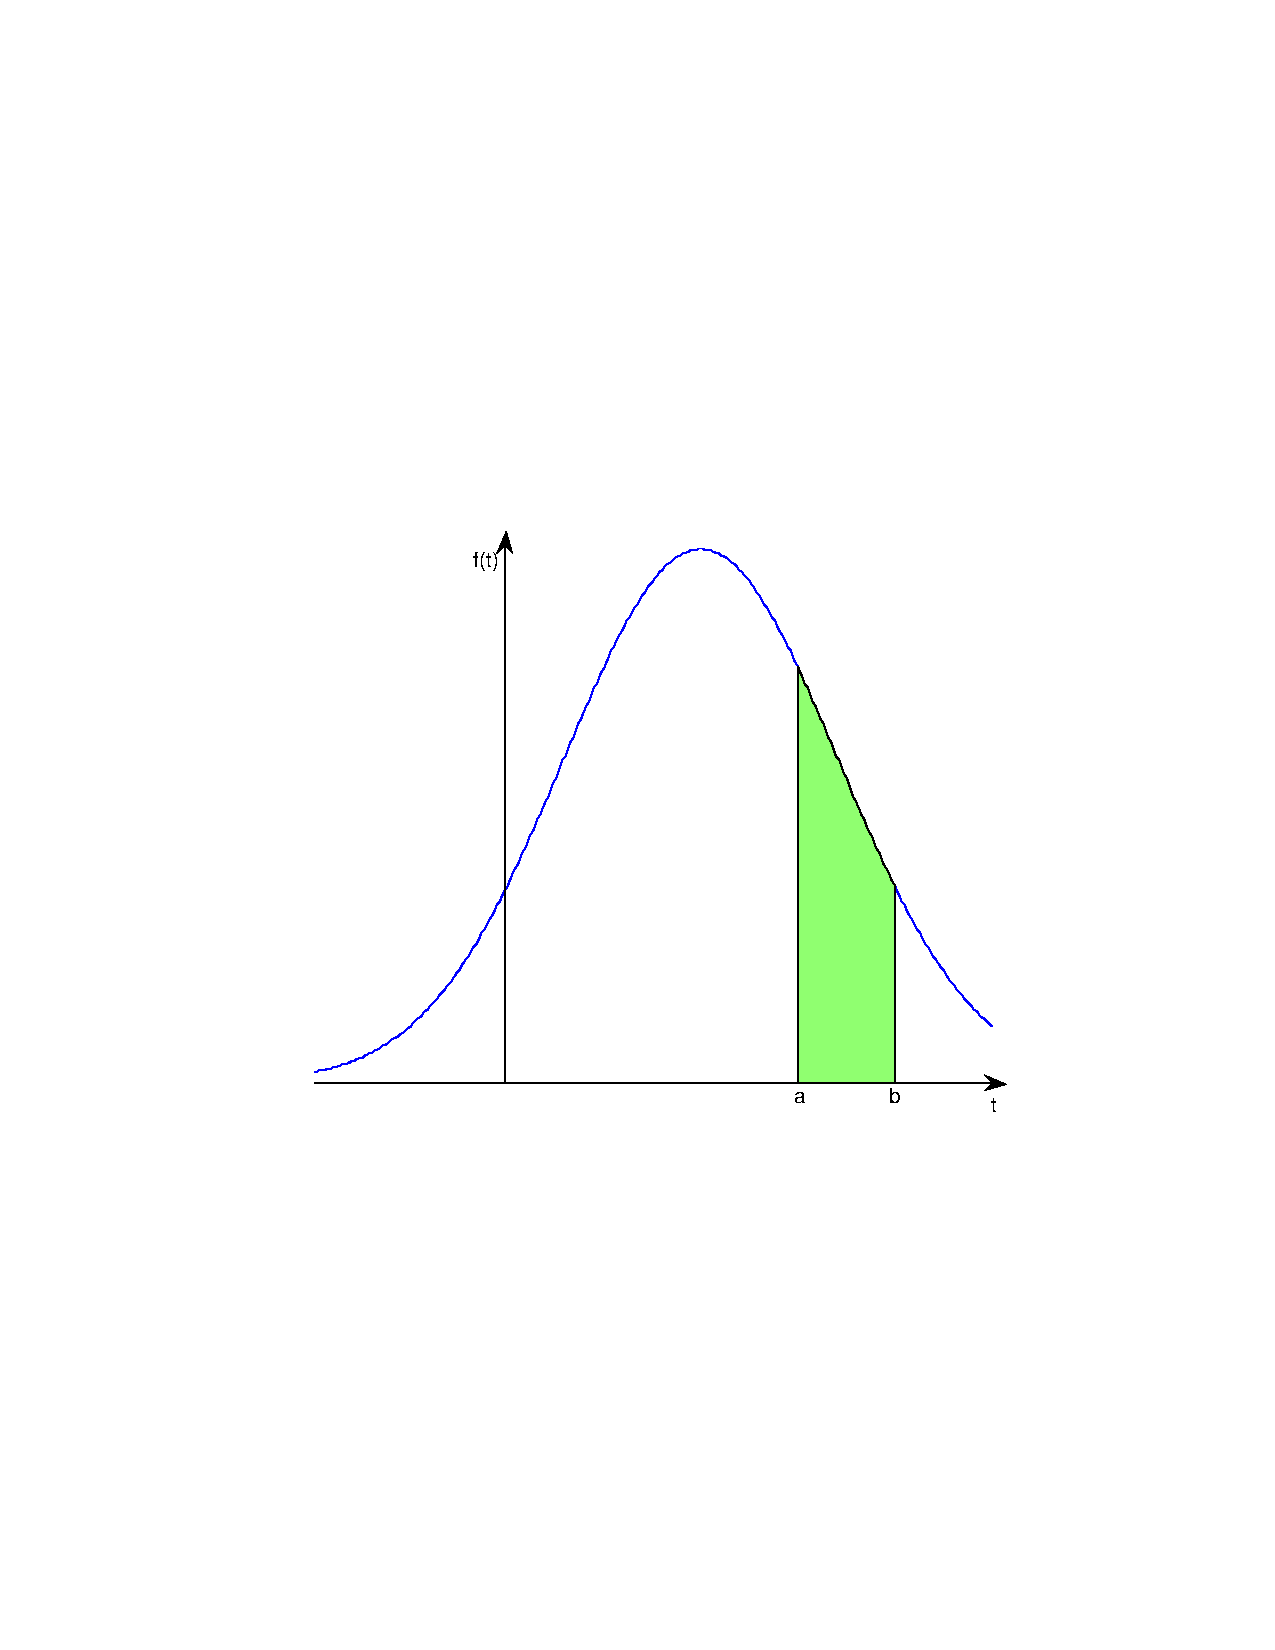
\includegraphics[width=0.5\textwidth]{FIGS/distrib_a_b}
\end{center}
\end{frame}

\begin{frame}\frametitle{Cumulative distribution function}
The cumulative distribution function (c.d.f.) is a function $F(t)$ that characterizes the distribution of $T$, and defined by
\[
F(s)=\IP(T\leq s)=\int_{-\infty}^sf(x)dx
\]
\begin{center}
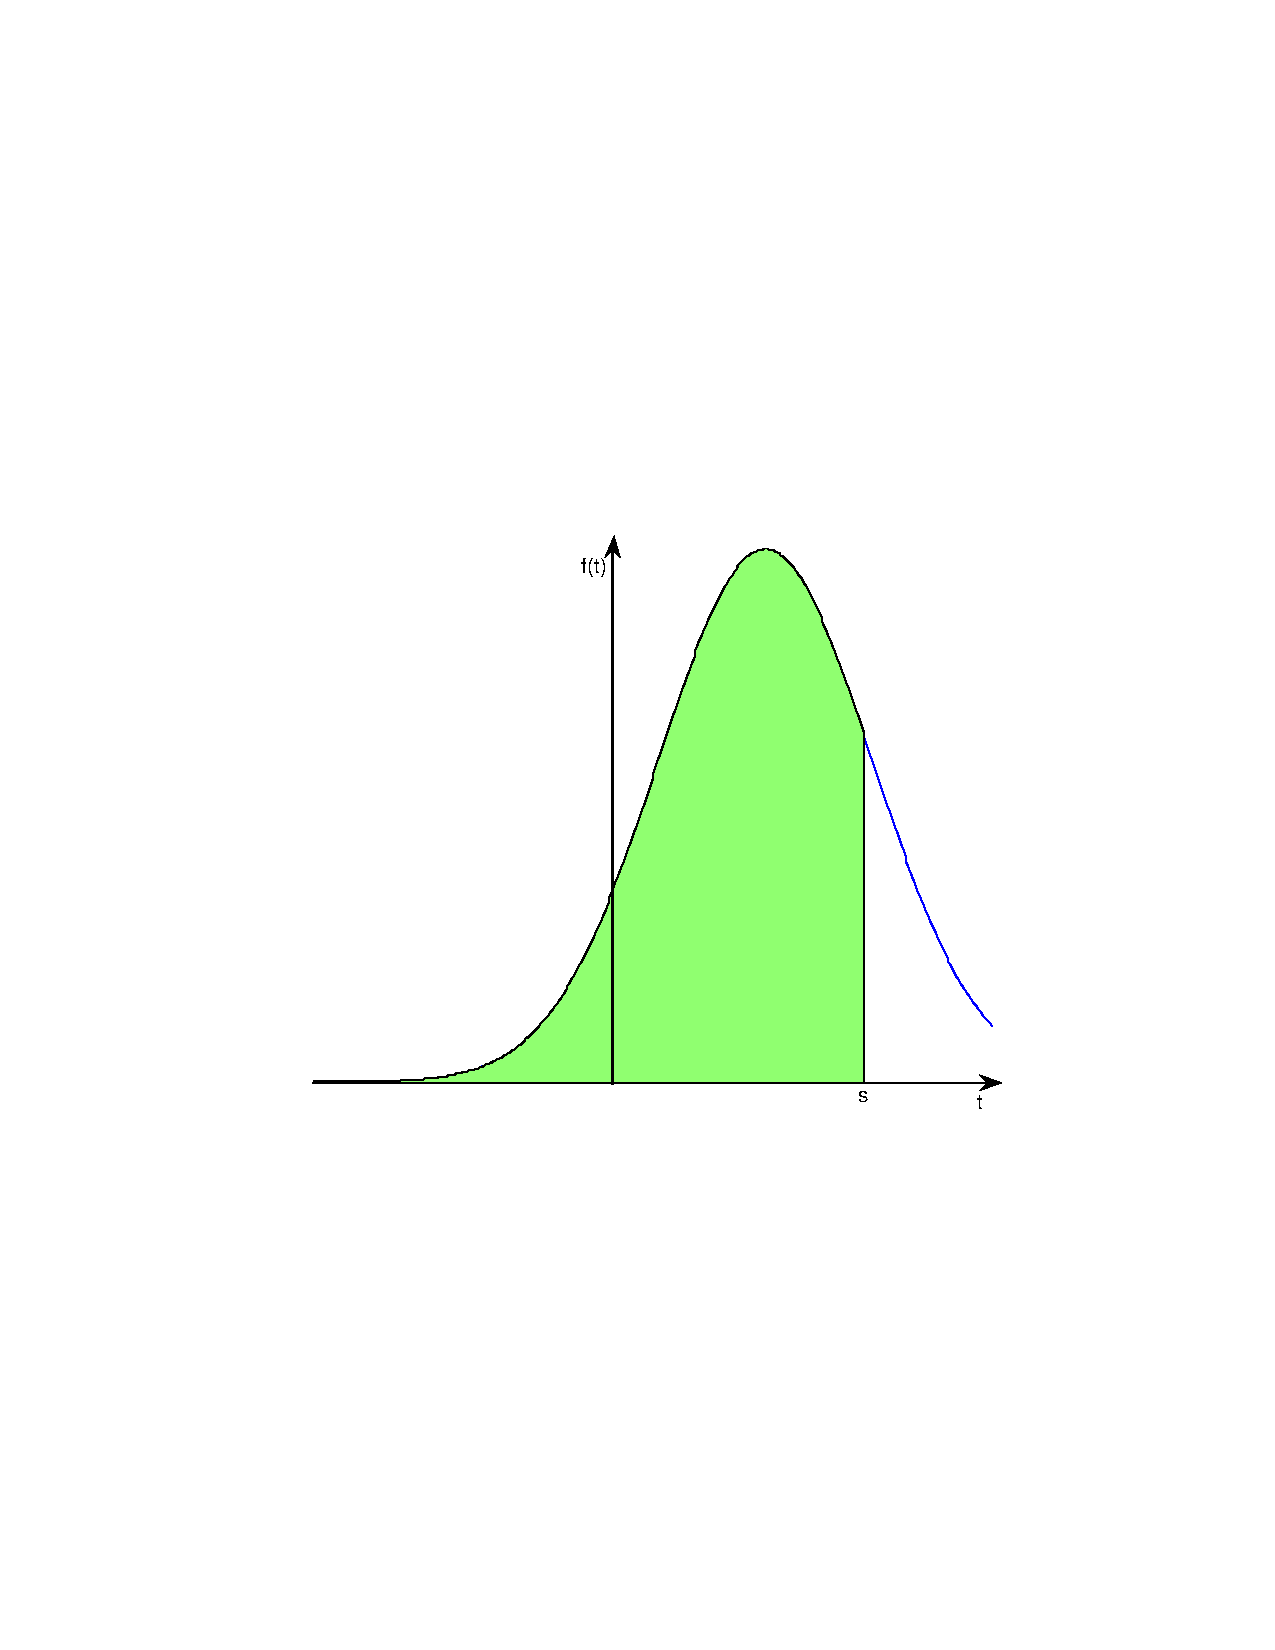
\includegraphics[width=0.5\textwidth]{FIGS/cdf_auc}
\end{center}
\end{frame}

\begin{frame}\frametitle{Survival function}
Another characterization of the distribution of the random variable $T$ is through the \defword{survival} (or \defword{sojourn}) function
\vfill
The survival function of state $S_0$ is given by 
\begin{equation}
  \S(t)=1-F(t)=\IP(T>t)
  \label{eq:survival}
\end{equation}
This gives a description of the \defword{sojourn time} of a
system in a particular state (the time spent in the state)
\vfill
$\S$ is a nonincreasing function (since $\S=1-F$
with $F$ a c.d.f.), and
$\S(0)=1$ (since $T$ is a nonnegative random variable)
\end{frame}

\begin{frame}
The \defword{average sojourn time} $\tau$ in state $S_0$ is given by
\[
\tau=E(T)=\int_0^\infty tf(t)dt
\]
Since $\lim_{t\to\infty}t\S(t)=0$, it follows that 
\[
\tau=\int_0^\infty \S(t)dt
\]
\vfill
\defword{Expected future lifetime}:
\[
\frac{1}{\S(t_0)} \int_0^{\infty} t\,f(t+t_0)\,dt 
\]
\vfill
\begin{eqnarray*}
\S(t)-\S(a)&=&\IP\left\{\textrm{survive during }
 (a,t)\textrm{ having survived until }a\right\} \\
&=& \exp\left(-\int_a^t h(u)du\right)
\end{eqnarray*}
\end{frame}

\begin{frame}\frametitle{Hazard rate}
The \defword{hazard rate} (or \defword{failure rate}) is
\begin{align*}
h(t) &= \lim_{\Delta t\to 0}\frac{\S(t)-\S(t+\Delta t)}{\Delta t} \\
& = \lim_{\Delta t\to 0} \frac{\IP{ T<t+\Delta t | T\geq
t}}{\Delta t} \\
&= \frac{f(t)}{\S(t)}
\end{align*}
It gives probability of failure between $t$ and $\Delta t$, given survival to $t$.
\vfill
We have
\[
h(t)=-\frac{d}{dt}\ln\S(t)
\]
\end{frame}

%%%%%%%%%%%%%%%%%%%%%%%%%%%
\begin{frame}{Competing risks}
Suppose now that the system starts in state $A$ at time $t=0$ and that depending on which of the two events $\mathcal{E}_1$ or $\mathcal{E}_2$ takes place first, it switches to state $B_1$ or $B_2$, respectively
\vfill
Consider the random variables $T_A$, \emph{time spent} in state $A$ (or sojourn time in $A$), $T_{AB_1}$, \emph{time before switch to} $B_1$ and $T_{AB_2}$, \emph{time before switch to} $B_2$
\vfill
If we consider state $A$, we cannot observe the variables $T_{AB_1}$ or $T_{AB_2}$. What is observable is the sojourn time in $A$
\[
T^*_A=\min\left( T_{AB_1},T_{AB_2} \right)
\]
(where $^*$ indicates that a quantity is observable)
\end{frame}

\begin{frame}{Failure rate by type of event}
We have two (or more) types of events whose individual failure rates have to be accounted for
\begin{align*}
h_j(t) &= \lim_{\Delta t\to 0} \frac{\mathbb{P}( T<t+\Delta t, S=S_j | T\geq t)}{\Delta t} 
\end{align*}
where $\mathbb{P}(T<t+\Delta t, S=S_j | T\geq t)$ is the probability of failure due to cause $S_j$ ($j=1,2$ ici), i.e., $S$ is a discrete r.v. representing the event that is taking place
\end{frame}

\begin{frame}
By the law of total probability, since only one of the event can take place, if there are $n$ risks, then
$$
h(t) = \sum_{i=1}^n h_j(t)
$$
or, identically,
$$
\mathcal{S}(t)
=
\exp\left(
  -\int_0^t \sum\textstyle_{j=1}^n h_j(s)\ ds
\right)
$$
\end{frame}

\begin{frame}
As a consequence, suppose a process is subject to two competing exponential risks with respective distributions with parameters $\theta_1$ and $\theta_2$
\vfill
Then the mean sojourn time in the initial state before being affected by one of the two risks is
$$
\frac{1}{\theta_1+\theta_2}
$$
\end{frame}


%%%%%%%%%%%%%%%%%%%
%%%%%%%%%%%%%%%%%%%
%%%%%%%%%%%%%%%%%%%
%%%%%%%%%%%%%%%%%%%
\subsection{Two ``extreme'' distributions and a nicer one}

\begin{frame}\frametitle{The exponential distribution}
The random variable $T$ has an \defword{exponential} distribution if its
probability density function takes the form
\begin{equation}\label{eq:exp_distrib}
f(t)=\begin{cases}0&\textrm{if }t<0,\\
\theta e^{-\theta t}&\textrm{if }t\geq 0,
\end{cases}
\end{equation}
with $\theta>0$. Then the
survival function for state $S_0$ is of the form $\S(t)=e^{-\theta
  t}$, for $t\geq 0$, and the average sojourn time in state $S_0$ is
\[
\tau=\int_0^\infty e^{-\theta t}dt=\frac 1\theta
\]
\end{frame}

\begin{frame}\frametitle{Particularities of the exponential distribution}
The standard deviation of an exponential distribution is also $1/\theta$. When estimating $\theta$, it is impossible to distinguish the mean and the standard deviation
\vfill
The exponential distribution is \defword{memoryless}: its conditional probability obeys
\[
P(T > s + t\; |\; T > s) = P(T > t),\quad\forall s, t \ge 0
\]

The exponential and geometric distributions are the only memoryless probability distributions
\vfill
The exponential distribution has a constant hazard function
\end{frame}

\begin{frame}\frametitle{The Dirac delta distribution}
If for some constant $\omega>0$,
\[
\S(t)=
\left\{
\begin{array}{ll}
1, & 0\leq t\leq\omega \\
0, & \omega<t
\end{array}
\right.
\]
meaning that $T$ has a Dirac delta distribution
$\delta_\omega(t)$, then the average sojourn time is
\[
\tau=\int_0^\omega dt=\omega
\]
with standard deviation $\sigma=0$
\end{frame}

\begin{frame}{The Gamma distribution}
R.v. $X$ is \defword{Gamma} distributed ($X\,\sim\Gamma(k, \theta)$) with \defword{shape parameter} $k$ and \defword{scale parameter} $\theta$ (or \defword{rate} $\beta = 1/\theta$) (all positive) if its probability density function takes the form
\begin{equation}\label{eq:gamma_distrib}
f(x;k,\theta) = \frac{x^{k-1} \mathrm{e}^{-\frac{x}{\theta}}}{\Gamma ( k)\theta ^k}
\end{equation}
where $x>0$ and $\Gamma$ is the Euler Gamma function, defined for all $z\in\mathbb{C}$ s.t. $\Re(z) > 0$ by
\[
\Gamma : z \mapsto \int_0^{+\infty}  t^{z-1}\,\mathrm{e}^{-t}\,\mathrm{d}t
\]
\end{frame}

\begin{frame}{Properties of the Gamma distribution}
Mean $k\theta$, variance $k\theta^2$
\vfill
Survival function
\[
\mathcal{S}(t)=
1-\frac{1}{\Gamma(k)}\gamma\left(
k,\frac{t}{\theta} 
\right)
=1-\frac{1}{\Gamma(k)}\gamma\left(
k,\beta t
\right)
\]
where 
\[
\gamma(a,x)=\int_0^x t^{a-1}{\rm e}^{-t}{\rm d}t
\]
is an incomplete Gamma function
\end{frame}


%%%%%%%%%%%%%%%%%%%
%%%%%%%%%%%%%%%%%%%
%%%%%%%%%%%%%%%%%%%
%%%%%%%%%%%%%%%%%%%
\subsection{A simple cohort model with death} 

\begin{frame}\frametitle{A model for a cohort with one cause of death}
Consider a \defword{cohort} of individuals born at the same time, e.g., the same year
\vfill
\begin{itemize}
\item At time $t=0$, there are initially $N_0>0$ individuals
\item All causes of death are compounded together 
\item The time until death, for a given individual, is a random variable $T$, with continuous probability density distribution $f(t)$ and survival function $P(t)$
\end{itemize}
\vfill
$N(t)$ the cohort population at time $t\geq 0$
\begin{equation}\label{eq:N_general}
N(t)=N_0P(t)
\end{equation}
\vfill
$P(t)$ proportion of initial population still alive at time $t$, so $N_0P(t)$ number in the cohort still alive at time $t$
\end{frame}

\begin{frame}\frametitle{Case where $T$ is exponentially distributed}
Suppose that $T$ has an exponential distribution with mean $1/d$ (or parameter $d$), $f(t)=de^{-dt}$. Then the survival function is $P(t)=e^{-dt}$, and \eqref{eq:N_general} takes the form
\begin{equation}\label{eq:N}
N(t)=N_0e^{-dt}
\end{equation}
\vfill
Now note that
\begin{align*}
\frac{d}{dt} N(t) &= -dN_0e^{-dt} \\
&= -dN(t)
\end{align*}
with $N(0)=N_0$.
\vfill
{\red $\Rightarrow$} The ODE $N'=-dN$ makes the assumption that the life expectancy at birth is exponentially distributed
\end{frame}



\begin{frame}
Survival function, $\S(t)=\IP(T>t)$, for an exponential distribution with mean 80 years
\begin{center}
\includegraphics[width=0.8\textwidth]{FIGS/course-03-prop_surviving_exp_80years}
\end{center}
\end{frame}


\begin{frame}\frametitle{Case where $T$ has a Dirac delta distribution}
Suppose that $T$ has a Dirac delta distribution at $t=\omega$, giving the
survival function 
\[
P(t)=\begin{cases}
1, & 0\leq t\leq\omega \\
0, & t>\omega 
\end{cases}
\]
Then \eqref{eq:N_general} takes the form
\begin{equation}\label{eq:N2}
N(t)=\begin{cases}
N_0, & 0\leq t\leq\omega \\
0, & t>\omega
\end{cases}
\end{equation}
All individuals survive until time $\omega$, then they all die at time $\omega$
\vfill
Here, $N'=0$ everywhere except at $t=\omega$, where it is undefined
\end{frame}




\begin{frame}
Survival function, $\S(t)=\IP(T>t)$, for a Dirac distribution with mean 80 years
\begin{center}
\includegraphics[width=0.8\textwidth]{FIGS/course-03-prop_surviving_dirac_80years}
\end{center}
\end{frame}




%%%%%%%%%%%%%%%%%%%
%%%%%%%%%%%%%%%%%%%
%%%%%%%%%%%%%%%%%%%
%%%%%%%%%%%%%%%%%%%
\subsection{A possible fix to the exponential distribution issue} 



\begin{frame}{Survival for the exponential distribution}
\begin{center}
\includegraphics[width=\textwidth]{FIGS/course-03-prop_surviving_exp_80years_details}
\end{center}
\end{frame}

\begin{frame}{Issues with the exponential distribution}
\bbullet Survival drops quickly
\vfill
\bbullet Survival continues way beyond the mean
\vfill
Acceptable if what matters is the average duration of sojourn in a compartment (e.g., long term dynamics)
\vfill
More iffy if one is interested in short-term dynamics
\vfill
\bbullet Exponential distribution with parameter $\theta$ has same mean and standard deviation $1/\theta$, i.e., a single parameter controls mean and dispersion about the mean
\end{frame}

\begin{frame}{Exponential distributions are bad but also cool}
$X_1$ and $X_2$ 2 i.i.d. (independent and identically distributed) r.v. with parametres $\theta_1$ and $\theta_2$. Then the probability density function of the r.v. $Z=X_1+X_2$ is given by the convolution
\begin{align}
 f_Z(z) &= \int_{-\infty}^\infty f_{X_1}(x_1) f_{X_2}(z - x_1)\,dx_1 \nonumber\\
   &= \int_0^z \theta_1 e^{-\theta_1 x_1} \theta_2 e^{-\theta_2(z - x_1)} \, dx_1 \nonumber\\
   &= \theta_1 \theta_2 e^{-\theta_2 z} \int_0^z e^{(\theta_2 - \theta_1)x_1}\,dx_1 \nonumber\\
   &= \begin{cases}
        \dfrac{\theta_1 \theta_2}{\theta_2-\theta_1} \left(e^{-\theta_1 z} - e^{-\theta_2 z}\right) & \text{ if } \theta_1 \neq \theta_2 \\
        \theta^2 z e^{-\theta z} & \text{ if } \theta_1 = \theta_2 =: \theta
      \end{cases}
\end{align}
\end{frame}

\begin{frame}{The tool we use}
\begin{theorem}
Let $X_i$ be independent exponentially distributed random variables with parameter $\xi$ and $Y = \sum_{i=1}^n X_i$
\vskip1cm
Then the random variable $Y\rightsquigarrow E(n,\xi)$, an Erlang distribution with \emph{shape} parameter $n$ and \emph{scale} parameter $\xi$
\end{theorem}
\vfill
(Erlang distribution: Gamma distribution with integer shape parameter)
\end{frame}

\begin{frame}{Consequences for compartmental models}
If $n$ compartments are traversed successively by individuals, with each compartment having an outflow rate of $1/\xi$ (or a mean sojourn time of $\xi$), then the time of sojourn from entry into the first compartment to exit from the last is Erlang distributed with mean $E(Y)=n\xi$ and variance $\mathsf{Var}(Y)=n\xi^2$
\vfill
\begin{center}
\def\skip{*3}
\begin{tikzpicture}[scale=0.5, 
every node/.style={transform shape},
auto,
box/.style={minimum size=1.5cm, 
draw=black, very thick},
draw, circle]
%% States (imported original variants)
\node [box, fill=gray!20] at (0\skip,8) (X) {$X$};
\node [box, fill=gray!20] at (0\skip,4) (X1) {$X_{1}$};
\node [box, fill=gray!20] at (1\skip,4) (X2) {$X_{2}$};
\node [box, fill=gray!20] at (3\skip,4) (Xk) {$X_{k}$};
\node [box, fill=gray!20] at (5\skip,4) (XNm1) {$X_{N-1}$};
\node [box, fill=gray!20] at (6\skip,4) (XN) {$X_{N}$};
% Metabox
\draw [blue,rounded corners, thick, fill=blue!40, fill opacity=0.2] (-0.5\skip,9) -- (7\skip,9) -- (7\skip, 7) -- (-0.5\skip, 7) -- cycle;
\draw [blue,rounded corners, thick, fill=blue!40, fill opacity=0.2] (-0.5\skip,5) -- (7\skip,5) -- (7\skip, 3) -- (-0.5\skip, 3) -- cycle;
%% Flows (exponential box)
\path [line, very thick] (X) to node [midway, above] (TextNode) {$\mu X$} (7\skip,8);
%% Flows (Erlang box)
\path [line, very thick] (X1) to node [midway, above] (TextNode) {$\varepsilon X_1$} (X2);
\path [line, very thick] (X2) to node [midway, above] (TextNode) {$\varepsilon X_2$} (2\skip,4);
\path [line, very thick] (4\skip,4) to node [midway, above] (TextNode) {$\varepsilon X_{N-2}$} (XNm1);
\path [line, very thick] (XNm1) to node [midway, above] (TextNode) {$\varepsilon X_{N-1}$} (XN);
\path [line, very thick] (XN) to node [midway, above] (TextNode) {$\varepsilon X_{N}$} (7\skip,4);
%% To and from centre node
\path [line, very thick, dashed] (2.25\skip,4) to node [midway, above] (TextNode) {} (Xk);
\path [line, very thick, dashed] (Xk) to node [midway, above] (TextNode) {} (3.75\skip,4);
%% Time lines
\draw [|-|, thick] (0\skip,6.5) -- (7\skip,6.5);
\draw [|-|, thick] (0\skip,2.5) -- (7\skip,2.5);
%% Labels of time lines 
\node at (6\skip,2) {Average sojourn time $N/\varepsilon$};
\node at (6\skip,6) {Average sojourn time $1/\mu$};
\end{tikzpicture}
\end{center}
\vfill
I have a \href{https://daytah-or-dahtah.ovh:3838/Erlang_shiny/}{Shiny app} for this :)
\end{frame}

\begin{frame}{Example: EVD incubation periods}
Consider the incubation period for Ebola Virus Disease. During the 2014 EVD crisis in Western Africa, the WHO Ebola Response Team estimated incubation periods in a 2015 paper
\vfill
Table S2 in the Supplementary Information in that paper gives the best fit for the distribution of incubation periods for EVD as a Gamma distribution with mean 10.3 days and standard deviation 8.2, i.e., $n\varepsilon = 10.3$ and $\varepsilon \sqrt{n}=8.2$
\vfill
From this, $\varepsilon = 8.2^2/10.3 \simeq 6.53$ and $n = 10.3^2/8.2^2 \simeq 1.57$. However, that is a Gamma distribution
\end{frame}

\begin{frame}[fragile]{Switching to a compartmental model approach}
To use multiple compartments to better fit residence times, we need to find the closest possible Erlang distribution to this Gamma distribution
\vfill
$\implies$ compute RSS errors between data points generated from the given Gamma distribution and an Erlang
\vfill 
\begin{knitrout}
\definecolor{shadecolor}{rgb}{0.969, 0.969, 0.969}\color{fgcolor}\begin{kframe}
\begin{alltt}
\hldef{error_Gamma} \hlkwb{<-} \hlkwa{function}\hldef{(}\hlkwc{theta}\hldef{,}\hlkwc{shape}\hldef{,}\hlkwc{t}\hldef{,}\hlkwc{d}\hldef{) \{}
  \hldef{test_points} \hlkwb{<-} \hlkwd{dgamma}\hldef{(t,} \hlkwc{shape} \hldef{= shape,} \hlkwc{scale} \hldef{= theta)}
  \hldef{ls_error} \hlkwb{<-} \hlkwd{sum}\hldef{((d}\hlopt{-}\hldef{test_points)}\hlopt{^}\hlnum{2}\hldef{)}
  \hlkwd{return}\hldef{(ls_error)}
\hldef{\}}
\end{alltt}
\end{kframe}
\end{knitrout}
\end{frame}

\begin{frame}[fragile]
\begin{knitrout}
\definecolor{shadecolor}{rgb}{0.969, 0.969, 0.969}\color{fgcolor}\begin{kframe}
\begin{alltt}
\hldef{optimize_gamma} \hlkwb{<-} \hlkwa{function}\hldef{(}\hlkwc{t}\hldef{,}\hlkwc{d}\hldef{) \{}
  \hldef{max_shape} \hlkwb{<-} \hlnum{10}
  \hldef{error_vector} \hlkwb{<-} \hlkwd{mat.or.vec}\hldef{(max_shape,}\hlnum{1}\hldef{)}
  \hldef{scale_vector} \hlkwb{<-} \hlkwd{mat.or.vec}\hldef{(max_shape,}\hlnum{1}\hldef{)}
  \hlkwa{for} \hldef{(i} \hlkwa{in} \hlnum{1}\hlopt{:}\hldef{max_shape) \{}
    \hldef{result_optim} \hlkwb{<-} \hlkwd{try}\hldef{(}\hlkwd{optim}\hldef{(}\hlkwc{par} \hldef{=} \hlnum{3}\hldef{,}
                              \hlkwc{fn} \hldef{= error_Gamma,}
                              \hlkwc{lower} \hldef{=} \hlnum{0}\hldef{,}
                              \hlkwc{method} \hldef{=} \hlsng{"L-BFGS-B"}\hldef{,}
                              \hlkwc{shape} \hldef{= i,}
                              \hlkwc{t} \hldef{= t,}
                              \hlkwc{d} \hldef{= d),}
                        \hlnum{TRUE}\hldef{)}
    \hlkwa{if} \hldef{(}\hlopt{!}\hlkwd{inherits}\hldef{(result_optim,}\hlsng{"try-error"}\hldef{)) \{}
      \hldef{error_vector[i]} \hlkwb{<-} \hldef{result_optim}\hlopt{$}\hldef{value}
      \hldef{scale_vector[i]} \hlkwb{<-} \hldef{result_optim}\hlopt{$}\hldef{par}
    \hldef{\}} \hlkwa{else} \hldef{\{}
      \hldef{error_vector[i]} \hlkwb{<-} \hlnum{NaN}
      \hldef{scale_vector[i]} \hlkwb{<-} \hlnum{NaN}
    \hldef{\}}
  \hldef{\}}
  \hldef{result_optim} \hlkwb{<-} \hlkwd{data.frame}\hldef{(}\hlkwd{seq}\hldef{(}\hlnum{1}\hldef{,max_shape),}
                             \hldef{scale_vector,}
                             \hldef{error_vector)}
  \hlkwd{colnames}\hldef{(result_optim)} \hlkwb{<-} \hlkwd{c}\hldef{(}\hlsng{"shape"}\hldef{,}\hlsng{"scale"}\hldef{,}\hlsng{"error"}\hldef{)}
  \hldef{result_optim} \hlkwb{<-} \hldef{result_optim[}\hlkwd{complete.cases}\hldef{(result_optim),]}
  \hlkwd{return}\hldef{(result_optim)}
\hldef{\}}
\end{alltt}
\end{kframe}
\end{knitrout}
\end{frame}


\begin{frame}[fragile]
\begin{knitrout}
\definecolor{shadecolor}{rgb}{0.969, 0.969, 0.969}\color{fgcolor}\begin{kframe}
\begin{alltt}
\hldef{time_points} \hlkwb{<-} \hlkwd{seq}\hldef{(}\hlnum{0}\hldef{,}\hlnum{60}\hldef{)}
\hldef{data_points} \hlkwb{<-} \hlkwd{dgamma}\hldef{(time_points,} \hlkwc{shape} \hldef{=} \hlnum{1.57}\hldef{,}
                      \hlkwc{scale} \hldef{=} \hlnum{6.53}\hldef{)}
\hlcom{# Run the minimization}
\hldef{optim_fits} \hlkwb{<-} \hlkwd{optimize_gamma}\hldef{(time_points,data_points)}
\hlcom{# Which is the best Erlang to fit the data}
\hldef{idx_best} \hlkwb{<-} \hlkwd{which.min}\hldef{(optim_fits}\hlopt{$}\hldef{error)}
\end{alltt}
\end{kframe}
\end{knitrout}
\end{frame}



\begin{frame}
Now plot the result as well as the original curve  (code chunk not shown)
\begin{center}
\includegraphics[width=\textwidth]{FIGS/course-03-plot_results_optim_Erlang}
\end{center}
\end{frame}






%%%%%%%%%%%%%%%%%%%
%%%%%%%%%%%%%%%%%%%
%%%%%%%%%%%%%%%%%%%
%%%%%%%%%%%%%%%%%%%
\subsection{Sojourn times in an SIS disease transmission model} 

\begin{frame}\frametitle{An SIS model}
\framesubtitle{Hypotheses}
\begin{itemize}
\item Individuals typically recover from the disease
\vfill
\item The disease does not confer immunity
\vfill
\item There is no birth or death (from the disease or natural) \newline\imply\;
Constant total population $N\equiv N(t)=S(t)+I(t)$
\vfill
\item Infection is of \defword{standard incidence} type
\end{itemize}
\end{frame}


\begin{frame}\frametitle{Recovery}
\begin{itemize}
\item Traditional models suppose that recovery occurs with rate constant
$\gamma$
\vfill
\item Here, of the individuals that become
infective at time $t_0$, a fraction $P(t-t_0)$ remain infective at
time $t\geq t_0$
\vfill
\item \imply\;
For $t\geq 0$, $P(t)$ is a survival function. As such, it verifies
$P(0)=1$ and $P$ is nonnegative and nonincreasing
\end{itemize}
\end{frame}


\begin{frame}\frametitle{Model for infectious individuals}
Since $N$ is constant, $S(t)=N-I(t)$ and we need only
consider the following equation (where $S$ is used for clarity)
\begin{equation}
I(t) = I_0(t)+ \int_0^t\beta\frac{S(u)I(u)}{N} P(t-u) du
\label{eq:SIS_I} 
\end{equation}
\vfill
\begin{itemize}
\item $I_0(t)$ number of individuals who were infective at time
$t=0$ and still are at time $t$
\begin{itemize}
\item $I_0(t)$ is nonnegative, nonincreasing, and
such that $\lim_{t\to\infty}I_0(t)=0$
\end{itemize}
\item $P(t-u)$ proportion of individuals who became infective at time $u$ and who still are at time $t$
\end{itemize}
\end{frame}


\begin{frame}\frametitle{Expression under the integral}
Integral equation for the number of infective individuals: 
\begin{equation}
I(t) = I_0(t)+ \int_0^t\beta\frac{(N-I(u))I(u)}{N} P(t-u) du
\tag{\ref{eq:SIS_I}} 
\end{equation}
The term
\[
\beta\frac{(N-I(u))I(u)}{N} P(t-u)
\]
\begin{itemize}
\item $\beta (N-I(u))I(u)/N$ is the rate at which new infectives are created, at time $u$
\item multiplying by $P(t-u)$ gives the proportion of those who became
infectives at time $u$ and who still are at time $t$
\end{itemize}
Summing over $[0,t]$ gives the number of infective individuals at time $t$
\end{frame}


\begin{frame}\frametitle{Case of an exponentially distributed time to recovery}
Suppose $P(t)$ such that sojourn time in the infective
state has exponential distribution with mean $1/\gamma$,
\textit{i.e.}, $P(t)=e^{-\gamma t}$
\vfill
Initial condition function $I_0(t)$ takes the form
\[
I_0(t)=I_0(0)e^{-\gamma t}
\]
with $I_0(0)$ the number of infective individuals at time $t=0$. Obtained by considering the cohort of initially infectious individuals, giving a
model such as \eqref{eq:N_general}
\vfill
Equation (\ref{eq:SIS_I}) becomes
\begin{equation}\label{eq:I_ODE}
I(t)=I_0(0)e^{-\gamma t}+\int_0^t \beta\frac{(N-I(u))I(u)}{N} e^{-\gamma
(t-u)}du
\end{equation}
\end{frame}

\begin{frame}
Taking the time derivative of \eqref{eq:I_ODE} yields
\begin{align*}
I'(t) &= -\gamma I_0(0)e^{-\gamma t}-\gamma\int_0^t
\beta\frac{(N-I(u))I(u)}{N}e^{-\gamma(t-u)}du \\
&\quad +\beta \frac{(N-I(t))I(t)}{N} \\
&= -\gamma\left(I_0(0)e^{-\gamma t}+
\int_0^t \beta\frac{(N-I(u))I(u)}{N}e^{-\gamma(t-u)}du\right) \\
&\quad +\beta \frac{(N-I(t))I(t)}{N} \\
&= \beta \frac{(N-I(t))I(t)}{N}-\gamma I(t)
\end{align*}
\vfill
This is the classical logistic type ordinary differential equation (ODE) for $I$ in an SIS model without vital dynamics (no birth or death)
\end{frame}



\begin{frame}\frametitle{Case of a step function survival function}
Consider case where the time spent infected has survival function 
\[
P(t)=\begin{cases}
1, & 0\leq t\leq\omega,\\
0, & t>\omega.
\end{cases}
\]
i.e., the sojourn time in the infective state is a constant
$\omega>0$
\vfill
In this case (\ref{eq:SIS_I}) becomes
\begin{equation}\label{eq:I_DDE}
I(t)=I_0(t)+\int_{t-\omega}^t \beta\frac{(N-I(u))I(u)}{N} du.
\end{equation}
Here, it is more difficult to obtain an expression for $I_0(t)$. It is however assumed that $I_0(t)$ vanishes for $t>\omega$
\end{frame}

\begin{frame}
When differentiated, \eqref{eq:I_DDE} gives, for $t\geq\omega$,
\[
I'(t)=I_0'(t)+\beta\frac{(N-I(t))I(t)}{N}
-\beta\frac{\left(N-I(t-\omega)\right)I(t-\omega)}{N}.
\]
Since $I_0(t)$ vanishes for $t>\omega$, this gives the delay
differential equation (DDE)
\[
I'(t)=\beta\frac{(N-I(t))I(t)}{N}
-\beta\frac{(N-I(t-\omega))I(t-\omega)}{N}.
\]
\end{frame}






%%%%%%%%%%%%%%%%%%%
%%%%%%%%%%%%%%%%%%%
\subsection{A model with vaccination}

\maxFrameImage{FIGS/ArinoCookePvdDVelasco.png}

%%%%%%%%%%%%%%%%%%%%%%%%%%
%%%%%%%%%%%%%%%%%%%%%%%%%%
\subsubsection{The general model}

\begin{frame}{A model with vaccine efficacy and waning}
\begin{itemize}
\item Exponential distribution of recovery times (rate $\gamma$)
\vfill
\item Susceptible individuals are vaccinated (number of vaccinated at time $t$ is denoted $V(t)$)
\vfill
\item Vaccination wanes, a fraction $P(t)$ of the vaccinated at time $t=0$ remain protected by the vaccine
\vfill
\item Vaccination is imperfect, $0\leq 1-\sigma\leq 1$ is the vaccine \defword{efficacy}
\end{itemize}
\end{frame}

\begin{frame}\frametitle{Model structure}
\centering
\def\skip{*2.5}
\begin{tikzpicture}[scale=1, transform shape]
%% Regular nodes
\node [circle, fill=green!50, text=black] at (0,0) (S) {$S$};
\node [circle, fill=red!90, text=black] at (2\skip,0) (I) {$I$};
\node [circle, fill=blue!50, text=black] at (1\skip,-2) (V) {$V$};
%% Fake nodes for arrows
\node [left=2cm of S] (birthS) {};
\node [left=1.5cm of V] (birthV) {};
\node [above=0.75cm of S] (dS) {};
\node [above=0.75cm of I] (dI) {};
\node [below=0.75cm of V] (dV) {};
%% Flows
\path [line, very thick] (birthS) to node [midway, above] (TextNode) {$(1-\alpha)dN$} (S);
\path [line, very thick] (birthV) to node [midway, below] (TextNode) {$\alpha dN$} (V);
\path [line, very thick] (S) to node [midway, right] (TextNode) {$dS$} (dS);
\path [line, very thick] (I) to node [midway, right] (TextNode) {$dI$} (dI);
\path [line, very thick] (V) to node [midway, right] (TextNode) {$dV$} (dV);
\path [line, very thick, bend left=10] (S) to node [midway, above] (TextNode) {$\beta SI/N$} (I);
\path [line, very thick, bend left=10] (I) to node [midway, below] (TextNode) {$\gamma I$} (S);
\path [line, very thick, bend left=10] (S) to node [midway,above,sloped] (TextNode) {$\phi S$} (V);
\path [line, very thick, bend left=10,color=red] (V) to node [midway,below,sloped] (TextNode) {$P(t)$} (S);
\path [line, very thick] (V) to node [midway, below, sloped] (TextNode) {$\sigma\beta VI/N$} (I);
\end{tikzpicture}    
\end{frame}

\begin{frame}\frametitle{Parametres}
\begin{itemize}
\item $d> 0$: mortality rate
\vfill
\item $\gamma\geq 0$: recovery rate
\vfill
\item $\beta> 0$: infectiousness of the disease
\vfill
\item $\phi\geq 0$: vaccination rate of susceptible individuals
\vfill
\item $\alpha\in[0,1)$: fraction of newborns vaccinates
\vfill
\item $0\leq 1-\sigma\leq 1$: efficacy of the vaccine. From now on, assume $0\leq \sigma< 1$
\end{itemize}
\end{frame}


\begin{frame}\frametitle{}
\begin{itemize}
\item Disease transmission: standard incidence
\vfill
\item Vaccination of newborns
\vfill
\item Birth and death rate equal (\imply constant total population)
\end{itemize}

\textbf{Assumptions on $P$}: $P(t)$ is a nonnegative and nonincreasing
function with $P(0^+)=1$, and such that $\int_0^\infty P(u)du$ is
positive and finite
\vfill
Constant total population $\Rightarrow$ $S(t)=N-I(t)-V(t)$; further, we
switch to \defword{proportions}: $S$, $I$ and $V$ represent the
proportions in the population, and $N=1$ ($S$ used in equations for
conciseness)
\end{frame}

\begin{frame}\frametitle{The SIS model with vaccination} 
\begin{subequations}\label{sys:SIVS_general}
\begin{align}
  \frac{dI(t)}{dt}&= \beta(S(t)+\sigma V(t))I(t)-(d+\gamma)I(t)
  \label{sys:SIVS_general_I}\\ 
  V(t)&= V_0(t) \label{sys:SIVS_general_V} \\
  &\quad +\int_0^t(\phi S(u)+\alpha d)P(t-u)e^{-d(t-u)}
  e^{-\sigma\beta\int_u^tI(x)dx}du \nonumber
\end{align}
\end{subequations}
\vfill
\begin{itemize}
\item $\alpha d$ proportion of vaccinated newborns
\item $\phi S(u)$ proportion of vaccinated susceptibles
\item $P(t-u)$ fraction of the proportion vaccinated still in the $V$
  class $t-u$ time units after going in
\item $e^{-d(t-u)}$ fraction of the proportion vaccinated
not dead due to natural causes
\item $e^{-\sigma\beta\int_u^t I(x)dx}$ fraction of the proportion
  vaccinated not gone to the infective class
\end{itemize} 
\end{frame}

\begin{frame}\frametitle{Obtaining the initial condition}
Let $v(t,\tau)$ be the (density) proportion of individuals in vaccination class-age $\tau$ still vaccinated at time $t$,
then
\begin{equation}\label{eq:SIVS_age_of_vaccination}
\left(\frac{\partial}{\partial t}+\frac{\partial}{\partial\tau}\right)
v(t,\tau)=
-(\sigma\beta I(t)+d+\eta(\tau))v(t,\tau)
\end{equation}
where $V(t)=\int_0^\infty v(t,\tau)d\tau$. $\eta(\tau)$ is the vaccine waning rate coefficient, with proportion still in the vaccination class-age $\tau$ being $P(\tau)=\exp\left(-\int_0^\tau\eta(q)dq\right)$.
It is assumed that $P$ is a survival function
\vfill
Inflow in class-age zero is 
\[
v(t,0)=\phi S(t)+\alpha d
\]
and $v(0,\tau)\geq 0$ is assumed
\end{frame}

\begin{frame}
Integrating \eqref{eq:SIVS_age_of_vaccination} along characteristics, dividing the integral for $V(t)$ at $t$, substituting in the solutions, and changing integration variables, we get
\begin{equation}
V_0(t)=e^{-\int_0^t(\sigma\beta I(x)+d)dx} \int_0^\infty
v(0,u)\frac{P(t+u)}{P(u)}du 
\label{eq:V0}
\end{equation}
The ratio $P(t+u)/P(u)=\exp\left(\int_u^{t+u}\eta(q)dq\right)$ is well defined for $t+u\geq u\geq 0$ and bounded above by 1
\vfill
Since $V(0)$ is finite, the integral in $V_0(t)$ converges, and thus $V_0(t)$ is nonnegative,
nonincreasing and $\lim_{t\to\infty}V_0(t)=0$
\end{frame}

\begin{frame}
Let
\[
\D=\{
(S,I,V); S\geq 0, I\geq 0, V\geq 0, S+I+V=1
\}
\]
\vfill
\begin{theorem}
The set $\D$ is positively invariant under the flow of \eqref{sys:SIVS_general} with $I(0)>0, S(0)>0$
\label{th:invariance_gen_model}
\end{theorem}
\end{frame}


\begin{frame}\frametitle{}
With the assumed initial conditions in $\D$, it can be shown that the system defined by \eqref{sys:SIVS_general_I} and \eqref{sys:SIVS_general_V} is equivalent to the system defined by \eqref{sys:SIVS_general_I} and
\begin{align}
\frac{d}{dt}V(t) &= \frac{d}{dt}V_0(t)+\phi S(t)+\alpha d \label{eq:Vprime_general} \\
&\quad -(d+\sigma\beta I(t))(V(t)-V_0(t)) 
+ Q(t)\nonumber
\end{align}
where to simplify notation, we denote
\[
Q(t)=\int_0^t (\phi S(u)+\alpha d) d_t(P(t-u))e^{-d(t-u)}
e^{-\sigma\beta\int_u^t I(x)dx}du
\]
\vfill
The system defined by \eqref{sys:SIVS_general_I} and \eqref{eq:Vprime_general} is of standard form, therefore results of Hale (see Hale \& Verduyn-Lunel) ensure the local existence, uniqueness and continuation of solutions of model \eqref{sys:SIVS_general}
\end{frame}

\begin{frame}\frametitle{$\R_0$}
Define $\R_0$ with vaccination as
\begin{equation}
\R_v=\R_0\left[
\frac{1+\sigma\phi\tilde P-(1-\sigma)\alpha d\tilde P}
{1+\phi\tilde P}
\right]
\label{eq:generalRphi}
\end{equation}
where $\R_0=\frac{\beta}{d+\gamma}$ is the reproduction number in the absence of vaccination and 
\[
\tilde P=\lim_{t\to\infty}\int_0^t P(v)e^{-dv}dv
\]
in such a way that $\tilde P<1/d$
\vfill
\bbullet
$\R_v\leq \R_0$ and, in absence of vaccination,
$\R_v=\R_0$
\end{frame}

\begin{frame}
\begin{theorem}
System \eqref{sys:SIVS_general} with an arbitrary loss of vaccination function $P(t)$ always admits the disease-free equilibrium
\begin{itemize}
\item
If $\R_0< 1$, then the DFE is the only equilibrium of the system and the disease goes extinct
\item
If $\R_v<1$, the DFE is LAS; if $\R_v>1$, the DFE is unstable
\end{itemize}
\label{th:R0_gen_mod}
\end{theorem}
\vfill
\begin{figure}[htbp]
 \begin{center}
   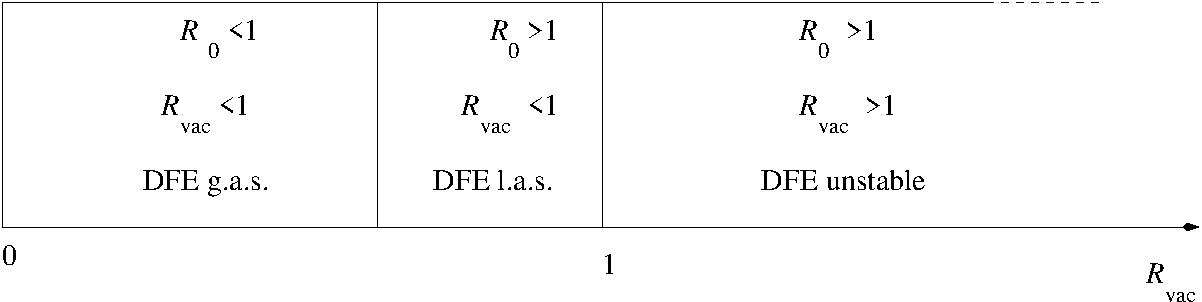
\includegraphics[width=0.95\textwidth]{FIGS/Rvac}
 \end{center}
\end{figure}
\end{frame}


%%%%%%%%%%%%%%%%%%%%%%%%%%
%%%%%%%%%%%%%%%%%%%%%%%%%%
\subsubsection{Case reducing to an ODE}

\begin{frame}\frametitle{Reduction of the system using specific $P(t)$ functions}
As before, two examples
\vfill
\begin{itemize}
\item The distribution of waning times is exponential, which leads to
 an ODE system. Treated briefly here, just so as to emphasize the
 presence of a so-called \emph{backward bifurcation}, a rather
 uncommon phenomenon in epidemiological models
\vfill
\item The waning time is a constant, which leads to a DDE model. We
 show that the backward bifurcation is also present
\end{itemize}
\end{frame}

\begin{frame}\frametitle{Case reducing to an ODE system}
Assume $P(v)=e^{-\theta v}$, $\theta>0$.
$V_0(t)=V_0(0)e^{-(d+\theta)t}e^{-\int_0^t\sigma\beta I(x)dx}$ from
(\ref{eq:V0}). Then (\ref{sys:SIVS_general_I}) and
(\ref{eq:Vprime_general}) give the ODE system
\begin{subequations}\label{ODEmodel}
\begin{align}
\frac{dI}{dt}&= \beta(1-I-(1-\sigma)V)I-(d+\gamma)I
\label{ODEmodelI}\\
\frac{dV}{dt}&= \phi(1-I-V)-\sigma\beta IV -(d+\theta)V+\alpha d
\label{ODEmodelV}
\end{align}
\end{subequations}
which with no newborn vaccination ($\alpha=0$) is the model studied in Kribs-Zaletta \& Velasco-Hernandez, 2000
\vfill
From Theorem~\ref{th:R0_gen_mod} the DFE always exists, with
\[
I_{DFE}=0,
S_{DFE}=\frac{\theta+d(1-\alpha)}{d+\theta+\phi},
V_{DFE}=\frac{\phi+\alpha d}{d+\theta+\phi}
\]
\end{frame}



\begin{frame}\frametitle{Backward bifurcation}
Assume that $\R_0>1$, then endemic equilibria (positive $I$
equilibria, denoted
by $I^\star$) can be obtained analytically from the quadratic equation
\[
\mathcal{P} (I)=AI^2+BI+C=0
\]
where
\begin{eqnarray*}
A&=& -\sigma\beta \\
B&=& \sigma(\beta-(d+\gamma))-(d+\theta+\sigma\phi)\\
C&=& (d+\gamma)(d+\theta+\phi)(\R_v-1)/\beta
\end{eqnarray*}
with
\[
\R_v=\R_0\frac{d+\theta+\sigma\phi-\alpha(1-\sigma)d}{d+\theta+\phi}
\]
from  (\ref{eq:generalRphi}).
\end{frame}

\begin{frame}
Backward bifurcation leading to two endemic
equilibria occurs for $\sigma>0$ if $ \mathcal{P}'(0)=B>0$,
$\mathcal{P}(0)=C<0$ and $B^2>4AC$ (we always have
$\mathcal{P}(1)<0$)
\vfill
\bbullet
On an $(\R_v,I)$ bifurcation diagram, this occurs for
$\R_c<\R_v<1$, where $\R_c$ is the value of $\R_v$ at
the saddle node bifurcation point where the two values of $I$ coincide,
\emph{i.e.}, $I=I_c=B/(-2A)$
\vfill
\bbullet
For $\R_v<\R_c$, there is no endemic equilibrium (EEP).
For $\R_v>1$, the constant term $C>0$, and there is a unique EEP
\vfill
\bbullet
In the case of forward bifurcation, $\R_c=1$; this is the case in
particular if the vaccine is totally effective ($\sigma=0$)
\end{frame}


\begin{frame}
By standard planar ODE arguments the following can be shown
\vfill
\begin{theorem}
For the ODE system (\ref{ODEmodel}) with $V(0)\geq 0$, $I(0)>0$, and $\R_0>1$
\vskip0.3cm
(i) if $\R_v<\R_c$, then the disease dies out
\vskip0.3cm
(ii) if $\R_c<\R_v<1$, then the EEP with larger $I$ is l.a.s., and the EEP with smaller $I$ is unstable
\vskip0.3cm
(iii) if $\R_v>1$, then the unique EEP is globally asymptotically stable in $\D\setminus\{I=0\}$
\label{th:odecase}
\end{theorem}
\end{frame}

\begin{frame}
Pertussis:
\begin{itemize}
\item 3 week average disease duration ($\gamma=0.04762$)
\item Average lifetime 75 years ($d=3.6530E-05$)
\item Average number of adequate contacts per infective per day is estimated at 0.4 ($\beta=0.4$)
\item Most newborns are vaccinated in the first few months of life
 ($\alpha=0.9$)
\item  Vaccine is effective, $\sigma=0.1$ (90\% effective vaccine).
\item Pertussis vaccine begins to wane after about 3 years
 and the average waning time of the vaccine
 $1/\theta$ is assumed to be 5 years, giving $\theta=5.4794E-04$
\end{itemize}
\vfill
With these parameter values, there is backward
bifurcation for a range of $\phi$ values given by $0.0254\leq\phi\leq0.1506$
\end{frame}

\begin{frame}
With the above parameter values, $\R_0=8.3936$ and
$\R_v(\phi)=0.8807$ for
$\phi=0.1$, which is in the range of backward bifurcation since the
critical value $\R_c(\phi)=0.8669<\R_v(\phi)<1$
\vfill
\begin{center}
   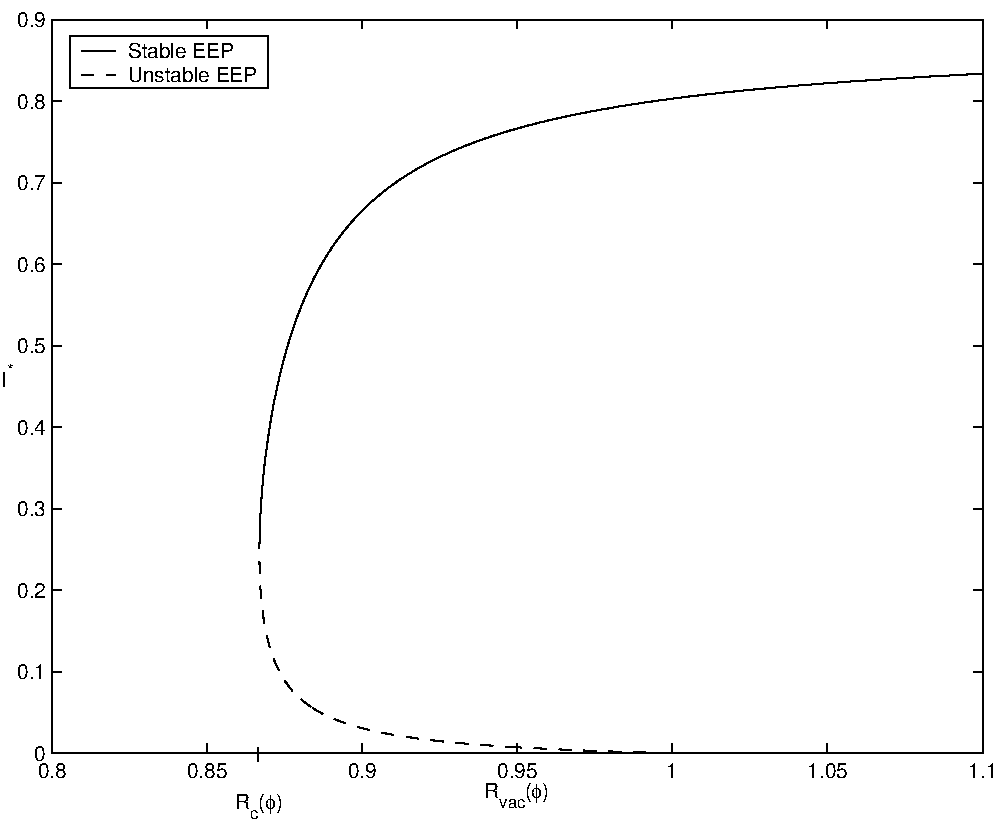
\includegraphics[width=0.8\textwidth]{FIGS/SIV_ode_bif_phi}
\end{center}
\end{frame}

%%%%%%%%%%%%%%%%%%%%%%%%%%
%%%%%%%%%%%%%%%%%%%%%%%%%%
\subsubsection{Case reducing to a DDE}
\begin{frame}\frametitle{Step function case: a delay integral model}
Suppose that
\[ 
P(v)=
\left\{
\begin{array}{l}
1\textrm{ if }v\in[0,\omega] \\
0\textrm{ otherwise} 
\end{array}
\right.
\]
Since $V_0(t)=0$ for $t>\omega$, with $S=1-I-V$ the
integral equation \eqref{sys:SIVS_general_V} becomes, for $t>\omega$
\begin{equation}
  V(t)=\int_{t-\omega}^t(\phi (1-I(u)-V(u))+\alpha d)e^{-d(t-u)}
  e^{-\sigma\beta\int_u^tI(x)dx}du
  \label{eq:VoftStepCase}
\end{equation}
\end{frame}

\begin{frame}
Differentiating \eqref{eq:VoftStepCase} (see equation
\eqref{eq:Vprime_general}) gives the model as the two
dimensional system, for $t>\omega$
\begin{subequations}\label{sys:SIVS_DDE}
\begin{align}
  \frac{d}{dt}I(t) &= 
  \beta(1-I(t)-(1-\sigma)V(t))I(t)-(d+\gamma)I(t) \label{sys:SIVS_DDE_dS} \\
  \frac{d}{dt}V(t) &=
  \phi(1-I(t)-V(t)) \label{sys:SIVS_DDE_dV}\\
  &\qquad-\phi(1-I(t-\omega)-V(t-\omega))e^{-d\omega}
  e^{-\sigma\beta\int_{t-\omega}^t I(x)dx} \nonumber \\
  &\qquad -\sigma\beta IV-dV
  +\alpha d\left(1-e^{-d\omega}e^{-\sigma\beta\int_{t-\omega}^t I(x)dx}
  \right) \nonumber
\end{align}
\end{subequations}
\vfill
Hereafter, shift time by $\omega$ so that these equations hold for $t>0$
\end{frame}


\begin{frame}
The well posedness of the problem follows from
Theorem~\ref{th:invariance_gen_model} and from the fact that solutions
of (\ref{sys:SIVS_general}) exist and are unique.
For a constant waning period, the basic reproduction number from
(\ref{eq:generalRphi}) is
\begin{equation}
 \R_v = \R_0
 \frac{d+(\sigma\phi-\alpha(1-\sigma)d)
 (1-e^{-d\omega})}{d+\phi(1-e^{-d\omega})}
 \label{eq:Rphi}
\end{equation}
\vfill
With $I_{DF}=0$, from Theorem~\ref{th:R0_gen_mod}
\begin{equation}
 V_{DF}=\frac{(\phi+\alpha d)(1-e^{-d\omega})}{d+\phi(1-e^{-d\omega})}
,\,\,
S_{DF}=\frac{d-\alpha d(1-e^{-d\omega})}{d+\phi(1-e^{-d\omega})}
 \label{eq:DFE_V}
\end{equation}
\end{frame}

\begin{frame}\frametitle{Finding the EEP's}
From nullclines, there exists one (or more) endemic equilbria
(EEP) iff there exists $0<I^\star\leq 1$ such that
\begin{equation}
 V^\star=f(I^\star)=g(I^\star)
 \label{eq:f_egal_g}
\end{equation}
where
\begin{equation}
 f(I)=\frac{1-1/\R_0-I}{1-\sigma}
 \label{eq:f(I)}
\end{equation}
for $\sigma<1$, and
\begin{equation}
 g(I)=\frac{(\phi(1-I)+\alpha d)(1-e^{-d\omega-\sigma\beta\omega I})}
 {\phi(1-e^{-d\omega-\sigma\beta\omega I})+d+\sigma\beta I}
 \label{eq:g(I)}
\end{equation}
\end{frame}


%%%%%%%%%%%%%%%%%%%
%%%%%%%%%%%%%%%%%%%
\begin{frame}
\frametitle{Visualising and locating the bifurcation}
From the nullcline equations, an EEP exists iff there exists an
$I^\star\in(0,1]$ such that equations (\ref{eq:f_egal_g})-(\ref{eq:g(I)})
hold.
So we study the zeros of
\[
H(I)=\frac{1-1/\R_0-I}{1-\sigma} -
\frac{(\phi(1-I)+\alpha d)(1-e^{-d\omega-\sigma\beta\omega I})}
{\phi(1-e^{-d\omega-\sigma\beta\omega I})+d+\sigma\beta I}
\]
To state the problem in a formal way, let
$\mathcal{A}=\{\alpha,\beta,\gamma,\omega,\phi,\sigma\}$ be the set of
parameters of interest, and denote
\begin{equation}
H(I,\mathcal{A})=
f(I)-g(I)
\label{eq:H}
\end{equation}
to show the dependence on these parameters.
\end{frame}

\begin{frame}
Proceed as follows
\begin{enumerate}
\item Choose a parameter $a_i\in\mathcal{A}$
\item Fix all other $a_j$'s ($j\neq i$)
\item Choose $a_{i,min}$, $a_{i,max}$ and $\Delta a_i$ for $a_i$
\item For all
  $a_{i,k}=a_{i,min}+k\Delta a_i$ ($k$
  such that $a_{i,k}\leq a_{i,max}$), compute
  $I^\star$ such that $H(I^\star,a_{i,k})=0$ \label{point1}
\end{enumerate}
Step~\ref{point1} is carried out using the {\sc MatLab} {\tt fzero} function
\vfill
Further precision can be gained by showing that
\[
H(0)=\frac{\R_v-1}{(1-\sigma)\R_0}
\]
and that, for $\sigma<1$
\[
H(1)=-\frac{1}{(1-\sigma)\R_0}-\frac{\alpha
d(1-e^{-d\omega-\sigma\beta\omega})}{\phi(1
-e^{-d\omega-\sigma\beta\omega})+d+\sigma\beta}<0
\]
\end{frame}

\begin{frame}
Define $\R_c$ as previously. For $\R_0>1$ and
$\R_v<1$, there are several possibilities
\begin{itemize}
\item If $\R_v<\R_c$, then there is no EEP. $H(0)$ and $H(1)$
 are strictly negative, and numerical simulations seem to indicate that $H$ has no roots in $(0,1]$ (\emph{i.e.}, that $H<0$ on this interval)
\item If $\R_c<\R_v<1$, then there are endemic equilibria.
 Here, since $H(0)$ and $H(1)$ are strictly negative, the only possibility is thus to have an even number of zeros of $H$. Numerical simulations appear to indicate that the number of endemic equilibria is 2
\end{itemize}
In between these two situations $\R_v=\R_c$ and there is one endemic equilibrium $I^\star$. Using the same procedure as for the visualisation of the bifurcation, it is possible to compute $\R_c$ by finding the value $I^\star$ such that
$H(I^\star,\mathcal{A})=0$ and $H'(I^\star,\mathcal{A})=0$, for a given parameter $a_i\in\mathcal{A}$
\vfill
If $\R_v>1$ then $H(0)>0$ and so there is an odd number of endemic equilibria. Numerical simulations indicate that there is a unique EEP
\end{frame}

\begin{frame}\frametitle{Numerical bifurcation analysis}
Same parameter values as in ODE case, except that the
constant waning time (the delay) $\omega$ has to be substituted for $\theta$. We take $\omega=1825$, \emph{i.e.}, corresponding to a 5 years waning time
\vfill
These parameters give $\R_0=8.3936$ and $\R_v(\phi)=0.8819$, which is in the range of the backward bifurcation since (using the above method) $\R_c(\phi)=0.8675$
\vfill
The bifurcation diagram is very like that depicted in earlier for the ODE. Numerical simulations of the DDE model (using {\tt dde23}) indicate that there are no additional bifurcations; solutions either go to the DFE or to the (larger) EEP
\end{frame}


\begin{frame}
\begin{center}
   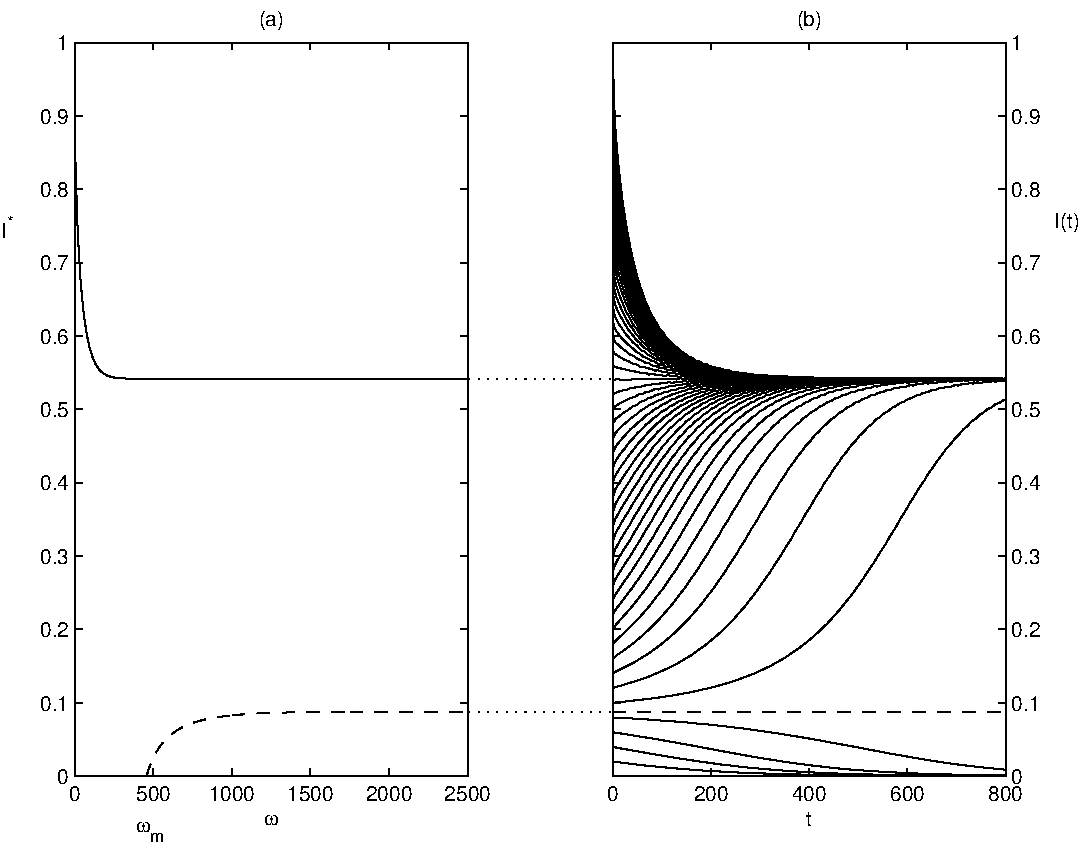
\includegraphics[width=0.75\textwidth]{FIGS/bif_and_time}
\end{center}
(a) Values of $I^\star$ as a function of $\omega$ by solving $H(I,\mathcal{A})=0$ with $a_i=\omega$. (b) Value of $I(t)$ versus time, obtained by numerical integration of system \eqref{sys:SIVS_DDE} with initial data $I(t)=c$, for $t\in[-\omega,0]$, $\omega=1825$, $c$ varying from 0 to 1 by steps of 0.02
\end{frame}

%%%%%%%%%%%%%%%%
%%%%%%%%%%%%%%%%
%%%%%%%%%%%%%%%%
%%%%%%%%%%%%%%%%
\subsection{Age of vaccination}
\begin{frame}\frametitle{Age of vaccination}
We have seen that infinite dimensionality can result from a detailed description (or an unspecified one) of the sojourn time in compartments
\vfill
We used age of vaccination to find the initial condition of \eqref{sys:SIVS_general}
\vfill
Here we take a closer look at this type of model
\vfill
Originally, age of infection was introduced to account for differences in infectivity depending on the time since an individual became infected
\vfill
For instance, it is known that infectiousness of HIV positive patients vary as a function of time
\end{frame}



\maxFrameImage{FIGS/BowmanArinoMoghadas-2011-cover.png}

\begin{frame}{How to model time between vaccine doses}
\begin{subequations}
\begin{align}
S\pprime &= -fS-V_1(t,0) \\
A\pprime &= \left(
(1-p)S+(1-p_1)\delta_1\tilde V_1+(1-p_2)\delta_2 V_2
\right)f-\mu_AA \\
I\pprime &= (pS+p_1\delta_1\tilde V_1+p_2\delta_2 V_2)f-\mu I \\
V_2\pprime &= V_1(t,a^\star)-\delta_2fV_2(t)
\end{align}
\begin{equation}\label{eq:V1_age_time}
\left(
\frac{\partial}{\partial t}+\frac{\partial}{\partial a}
\right) V_1(t,a) = -\delta_1fV_1(t,a),\quad 0\leq a\leq a^\star
\end{equation}
and boundary condition
\begin{equation}
V_1(t,0) = \begin{cases}
\gamma S_0\left(\frac{S(t)}{S(t)+A(t)}\right) & \text{if } T\leq t\leq T_e \text{ and }S>0 \\
0 & \text{otherwise}
\end{cases}
\end{equation}
\end{subequations}
where $f=\beta(\delta_AA+I)$ and $\tilde V_1(t)=\int_0^{a^\star}V_1(t,a)da$
\end{frame}

\begin{frame}{Simplifying a bit}
Integrate \eqref{eq:V1_age_time} using characteristics along lines $a=s$ and $t=T+s$, with $s$ as a new variable
\begin{equation}\label{eq:V1_age_time_integrated}
V_1(t,a)=V_1(t-a,0)\exp\left(\int_{t-a}^t -\delta_1f(\xi)\ d\xi\right)
\end{equation}
Define
\[
\zeta(t)=\int_0^t\delta_1f(\xi)d\xi
\]
and substitute into \eqref{eq:V1_age_time_integrated}, giving
\[
V_1(t,a)=V_1(t-a,0)\exp\left(\zeta(t-a)\zeta(t)\right)
\]
So the distributed delay is now discrete
\end{frame}

\begin{frame}{Simplifying a bit more}
Let
\[
\nu(t)=\int_0^t V_1(s,0)e^{\zeta(s)}ds
\]
Then the total number of individuals having been vaccinated with a single dose is
\[
\tilde V_1(t)=e^{-\zeta(t)}
\left(
\nu(t)-\nu(t-a^\star)
\right)
\]
\begin{subequations}
\begin{align}
S\pprime &= -fS-V_1(t,0) \\
A\pprime &= \left(
(1-p)S+(1-p_1)\delta_1\tilde V_1+(1-p_2)\delta_2 V_2
\right)f-\mu_AA \\
I\pprime &= (pS+p_1\delta_1\tilde V_1+p_2\delta_2 V_2)f-\mu I \\
V_2\pprime &= V_1(t-a^\star,0)e^{\zeta(t-a^\star)}-\delta_2fV_2(t) \\
\zeta\pprime &= \delta_1f \\
\nu\pprime &= V_1(t,0)e^{\zeta(t)}
\end{align}
\end{subequations}
\end{frame}

%%%%%%%%%%%%%%%%%%%
%%%%%%%%%%%%%%%%%%%
%%%%%%%%%%%%%%%%%%%
%%%%%%%%%%%%%%%%%%%
\subsection{Conclusions on sojourn times}

\begin{frame}\frametitle{Conclusions on sojourn times}
\begin{itemize}
\item The time of sojourn in compartments plays an important role in determining the type of model that we deal with
\vfill
\item All ODE models, when they use terms of the form $\kappa X$, make the assumption that the time of sojourn in compartments is exponentially distributed with parameter $\kappa$
\vfill
\item At the other end of the spectrum, delay differential with discrete delay make the assumption of a constant sojourn time, equal for all individuals
\vfill
\item Both can be true sometimes... but reality is more likely somewhere in between
\end{itemize}
\end{frame}



%%%%%%%%%%%%%%%%%%%
%%%%%%%%%%%%%%%%%%%
%%%%%%%%%%%%%%%%%%%
%%%%%%%%%%%%%%%%%%%
\section{Continuous time Markov chains}

\begin{frame}{Continuous-time Markov chains}
    CTMC similar to DTMC except in way they handle time between events (transitions)
\vfill
    DTMC: transitions occur each $\Delta t$
   \vfill 
    CTMC: $\Delta t\to 0$ and transition times follow an exponential distribution parametrised by the state of the system
    \vfill
    CTMC are roughly equivalent to ODE    
\end{frame}


\subsection{ODE $\leftrightarrow$ CTMC}

\begin{frame}{Converting your compartmental ODE model to CTMC}
    Easy as $\pi$ :)
\vfill
\begin{itemize}
    \item Compartmental ODE model focuses on flows into and out of compartments
    \vfill
    \item ODE model has as many equations as there are compartments
    \vfill
    \item Compartmental CTMC model focuses on transitions
    \vfill
    \item CTMC model has as many transitions as there are arrows between (or into or out of) compartments
\end{itemize}
\end{frame}


\begin{frame}{ODE to CTMC : focus on different components}
    \begin{center}
        \begin{tikzpicture}[auto,
            scale=1.2, every node/.style={transform shape},
            cloud/.style={minimum width={width("N-1")+2pt},
            draw, ellipse,fill=red!20}]
            \node[cloud, fill=green!90, double=red] (S) at (0,0) {$S$};
            \node[cloud, draw=none, fill=white] (h4) at (2,0) {};
            \node[cloud, fill=red!90, double=red] (I) at (4,0) {$I$};
            \node[cloud, fill=green!90] (S2) at (6,0) {$S$};
            \node[cloud, fill=red!90] (I2) at (8,0) {$I$};
            %% Flows (ODE)
            \path [line, bend left, very thick, dashed] (S) to node [midway, above] (TextNode) {$-\beta SI$} (h4);
            \path [line, bend left, very thick] (h4) to node [midway, below] (TextNode) {$+\gamma I$} (S);
            \path [line, bend left, very thick] (h4) to node [midway, above] (TextNode) {$+\beta SI$} (I);
            \path [line, bend left, very thick, dashed] (I) to node [midway, below] (TextNode) {$-\gamma I$} (h4);
            %% Flows (CTMC)
            \path [line, bend left, very thick, red] (S2) to node [midway, above, black] (TextNode) {$\beta SI$} (I2);
            \path [line, bend left, very thick, red] (I2) to node [midway, below] (TextNode) {$\gamma I$} (S2);
            %%
            \draw[very thick, dotted] (5,-2) -- (5,2);
            %%
            \node[style=rectangle] at (2,2) {ODE};
            \node[style=rectangle] at (7,2) {CTMC};
            %%
            \node[style=rectangle] (fODE) at (2,-2) {focus};
            \path [line, dotted,red] (fODE) to  (S.south);
            \path [line, dotted,red] (fODE) to  (I.south);
            \node[style=rectangle] (fCTMC) at (6,-2) {focus};
            \path [line, dotted,red] (fCTMC) to (6.75,0.3);
            \path [line, dotted,red] (fCTMC) to  (6.75,-0.475);
        \end{tikzpicture}        
    \end{center}
\end{frame}


\begin{frame}{SIS without demography}
    \begin{center}
        \begin{tabular}{cp{3cm}cc}
          \toprule
            Transition & Effect & Weight & Probability \\
            \midrule
            $S\to S-1$, $I\to I+1$ & new infection & $\beta SI$ & $\dfrac{\beta SI}{\beta SI+\gamma I}$ \\
            $S\to S+1$, $I\to I-1$ & recovery of an infectious & $\gamma I$ & $\dfrac{\gamma I}{\beta SI+\gamma I}$ \\
            \bottomrule
        \end{tabular}
    \end{center}
    \vfill
    States are $S,I$
\end{frame}


\begin{frame}{SIS with demography}
    \begin{center}
        \begin{tabular}{p{3cm}p{3cm}cc}
        \toprule
            Transition & Effect & Weight & Probability \\
          \midrule
            $S\to S+1$ & birth of a susceptible & $b$ & $\frac{b}{b+d(S+I)+\beta SI+\gamma I}$ \\
            $S\to S-1$ & death of a susceptible & $dS$ & $\frac{dS}{b+d(S+I)+\beta SI+\gamma I}$ \\
            $S\to S-1$, $I\to I+1$ & new infection & $\beta SI$ & $\frac{\beta SI}{b+d(S+I)+\beta SI+\gamma I}$ \\
            $I\to I-1$ & death of an infectious & $dI$ & $\frac{dI}{b+d(S+I)+\beta SI+\gamma I}$ \\
            $S\to S+1$, $I\to I-1$ & recovery of an infectious & $\gamma I$ & $\frac{\gamma I}{b+d(S+I)+\beta SI+\gamma I}$ \\
            \bottomrule
        \end{tabular}
    \end{center}
\vfill
States are $S,I$
\end{frame}


\begin{frame}[fragile]{Kermack \& McKendrick model}
    \begin{center}
        \begin{tabular}{cp{3cm}cc}
        \toprule
            Transition & Effect & Weight & Probability \\
            \midrule
            $S\to S-1$, $I\to I+1$ & new infection & $\beta SI$ & $\dfrac{\beta SI}{\beta SI+\gamma I}$ \\
            $I\to I-1$, $R\to R+1$ & recovery of an infectious & $\gamma I$ & $\dfrac{\gamma I}{\beta SI+\gamma I}$ \\
            \bottomrule
        \end{tabular}
    \end{center}
    \vfill
    States are $S,I,R$
\end{frame}


\subsection{Simulating CTMC (in theory)}

\begin{frame}{Gillespie's algorithm}
    \begin{itemize}
        \item A.k.a. the stochastic simulation algorithm (SSA)
        \vfill
        \item Derived in 1976 by Daniel Gillespie
        \vfill
        \item Generates possible solutions for CTMC
        \vfill
        \item Extremely simple, so worth learning how to implement; there are however packages that you can use (see later)
    \end{itemize}
\end{frame}


\begin{frame}{Gillespie's algorithm}
Suppose system has state $\mathbf{x}(t)$ with initial condition $\mathbf{x}(t_0)=\mathbf{x}_0$ and \emph{propensity functions} $a_i$ of elementary reactions
\vfill
set $t\leftarrow t_0$ and $\mathbf{x}(t)\leftarrow \mathbf{x}_0$\\
while {$t\leq t_f$}\\
- $\xi_t\leftarrow \sum_j a_j(\mathbf{x}(t))$\\
- Draw $\tau_t$ from $T\thicksim \mathcal{E}(\xi_t)$\\
- Draw $\zeta_t$ from $\mathcal{U}([0,1])$\\
- Find $r$, smallest integer s.t. $\sum_{k=1}^j a_k(\mathbf{x}(t))> \zeta_t\sum_j a_j(\mathbf{x}(t))=\zeta_t\xi_t$\\
- Effect the next reaction (the one indexed $r$)\\
- $t\leftarrow t+\tau_t$\\    
\end{frame}


\begin{frame}{Drawing at random from an exponential distribution}
    If you do not have an exponential distribution random number generator.. We want $\tau_t$ from $T\thicksim\mathcal{E}(\xi_t)$, i.e., $T$ has probability density function
    $$
    f(x,\xi_t)=
    \xi_te^{-\xi_t x}\mathbf{1}_{x\geq 0}
    $$
    Use cumulative distribution function $F(x,\xi_t)=\int_{-\infty}^x f(s,\xi_t)\,ds$
    $$
    F(x,\xi_t)=
    (1-e^{-\xi_t x})\mathbf{1}_{x\geq 0}
    $$
    which has values in $[0,1]$. So draw $\zeta$ from $\mathcal{U}([0,1])$ and solve $F(x,\xi_t)=\zeta$ for $x$
    \begin{align*}
    F(x,\xi_t)=\zeta & \Leftrightarrow 1-e^{-\xi_tx}=\zeta \\
    &\Leftrightarrow e^{-\xi_tx} = 1-\zeta \\
    &\Leftrightarrow \xi_tx = -\ln(1-\zeta) \\
    &\Leftrightarrow \boxed{x = \frac{-\ln(1-\zeta)}{\xi_t}}
    \end{align*}
\end{frame}


\begin{frame}{Gillespie's algorithm (SIS model with only I eq.)}
set $t\leftarrow t_0$ and $I(t)\leftarrow I(t_0)$\\
while {$t\leq t_f$}\\
- $\xi_t\leftarrow \beta (P^\star-i)i+\gamma i$\\
- Draw $\tau_t$ from $T\thicksim \mathcal{E}(\xi_t)$\\
- $v\leftarrow\left[\beta (P^\star-i)i,\xi_t\right]/\xi_t$\\
- Draw $\zeta_t$ from $\mathcal{U}([0,1])$\\
- Find $pos$ such that $v_{pos-1}\leq\zeta_t\leq v_{pos}$\\
- switch {$pos$}\\
\qquad - 1: New infection, $I(t+\tau_t)=I(t)+1$ \\
\qquad - 2: End of infectious period, $I(t+\tau_t)=I(t)-1$ \\
- $t\leftarrow t+\tau_t$
\end{frame}


\begin{frame}{Sometimes Gillespie goes bad}
    \begin{itemize}
        \item Recall that the inter-event time is exponentially distributed
        \item Critical step of the Gillespie algorithm:
        \begin{itemize}
            \item $\xi_t\leftarrow$ weight of all possible events (\emph{propensity})
            \item Draw $\tau_t$ from $T\thicksim \mathcal{E}(\xi_t)$
        \end{itemize}
        \item So the inter-event time $\tau_t\to 0$ if $\xi_t$ becomes very large for some $t$
        \item This can cause the simulation to grind to a halt
    \end{itemize}
\end{frame}


\begin{frame}{Example: a birth and death process}
    \begin{itemize}
        \item Individuals born at \emph{per capita} rate $b$
        \item Individuals die at \emph{per capita} rate $d$
        \item Let's implement this using classic Gillespie
    \end{itemize}
    \vfill
(See \href{https://raw.githubusercontent.com/julien-arino/3MC-course-epidemiological-modelling/main/CODE/simulate_birth_death_CTMC.R}{\code{simulate\_birth\_death\_CTMC.R}} on course GitHub repo)
\end{frame}


\begin{frame}{Gillespie's algorithm (birth-death model)}
set $t\leftarrow t_0$ and $N(t)\leftarrow N(t_0)$\\
while {$t\leq t_f$}\\
- $\xi_t\leftarrow (b+d)N(t)$\\
- Draw $\tau_t$ from $T\thicksim \mathcal{E}(\xi_t)$\\
- $v\leftarrow\left[bN(t),\xi_t\right]/\xi_t$\\
- Draw $\zeta_t$ from $\mathcal{U}([0,1])$\\
- Find $pos$ such that $v_{pos-1}\leq\zeta_t\leq v_{pos}$\\
- switch {$pos$}\\
\qquad - 1: Birth, $N(t+\tau_t)=N(t)+1$ \\
\qquad - 2: Death, $N(t+\tau_t)=N(t)-1$ \\
- $t\leftarrow t+\tau_t$    
\end{frame}

% <<>>=
% b = 0.01   # Birth rate
% d = 0.01   # Death rate
% t_0 = 0    # Initial time
% N_0 = 100  # Initial population
% 
% # Vectors to store time and state. Initialise with initial condition.
% t = t_0
% N = N_0
% 
% t_f = 1000  # Final time
% 
% # We'll track the current time and state (could also just check last entry in t
% # and N, but will take more operations)
% t_curr = t_0
% N_curr = N_0
% while (t_curr<=t_f) {
%     xi_t = (b+d)*N_curr
%     # The exponential number generator does not like a rate of 0 (when the 
%     # population crashes), so we check if we need to quit
%     if (N_curr == 0) {
%         break
%     }
%     tau_t = rexp(1, rate = xi_t)
%     t_curr = t_curr+tau_t
%     v = c(b*N_curr, xi_t)/xi_t
%     zeta_t = runif(n = 1)
%     pos = findInterval(zeta_t, v)+1
%     switch(pos,
%             { 
%                 N_curr = N_curr+1 # Birth
%             },
%             {
%                 N_curr = N_curr-1 # Death
%             })
%     N = c(N, N_curr)
%     t = c(t, t_curr)
% }
% @

\begin{frame}[fragile]
\begin{lstlisting}[language=Renhanced]
b = 0.01   # Birth rate
d = 0.01   # Death rate
t_0 = 0    # Initial time
N_0 = 100  # Initial population

# Vectors to store time and state. Initialise with initial condition.
t = t_0
N = N_0

t_f = 1000  # Final time

# We'll track the current time and state (could also just check last entry in t
# and N, but will take more operations)
t_curr = t_0
N_curr = N_0
\end{lstlisting}
\end{frame}

\begin{frame}[fragile]
\begin{lstlisting}[language=Renhanced]
while (t_curr<=t_f) {
    xi_t = (b+d)*N_curr
    # The exponential number generator does not like a rate of 0 (when the 
    # population crashes), so we check if we need to quit
    if (N_curr == 0) {
        break
    }
    tau_t = rexp(1, rate = xi_t)
    t_curr = t_curr+tau_t
    v = c(b*N_curr, xi_t)/xi_t
    zeta_t = runif(n = 1)
    pos = findInterval(zeta_t, v)+1
    switch(pos,
            { 
                N_curr = N_curr+1 # Birth
            },
            {
                N_curr = N_curr-1 # Death
            })
    N = c(N, N_curr)
    t = c(t, t_curr)
}
\end{lstlisting}
\end{frame}

\maxFrameImage{FIGS/CTMC_birth_death_sol_b=0_01_d=0_01}
\maxFrameImage{FIGS/CTMC_birth_death_sol_b=0_01_d=0_02}
\maxFrameImage{FIGS/CTMC_birth_death_sol_b=0_03_d=0_01}


\begin{frame}[fragile]{Last one did not go well}
    \begin{itemize}
        \item Wanted 1000 time units (days?)
        \item Interrupted at $t=344.4432$ because I lost patience
        \newline (Penultimate slide: sim stopped because the population went extinct, I did not stop it!)
        \item At stop time
        \begin{itemize}
            \item $N = 103,646$
            \item $|N| = 208,217$ (and $|t|$ as well, of course!)
            \item time was moving slowly
        \end{itemize}
    \end{itemize}
    \vfill
    \begin{lstlisting}
> tail(diff(t))
[1] 1.282040e-05 5.386999e-04 5.468540e-04 1.779985e-04 6.737294e-05 2.618084e-04
    \end{lstlisting}
\end{frame}


\maxFrameImage{FIGS/CTMC_birth_death_ie_vs_t_b=0_03_d=0_01}

\subsection{Simulating CTMC (in practice)}

\begin{frame}{Tau-leaping (and packages) to the rescue!}
    \begin{itemize}
        \item \emph{Approximation} method (compared to classic Gillespie, which is exact)
        \item Roughly: consider "groups" of events instead of individual events
        \item Good news: \code{GillespieSSA2} and \code{adaptivetau}, two standard packages for SSA in \code{R}, implement tau leaping
    \end{itemize}
\end{frame}

% <<sim-gillespie2-first,echo=FALSE>>=
% library(GillespieSSA2)
% Pop <- 1000
% I_0 <- 2
% IC <- c(S = (Pop-I_0), I = I_0)
% params <- c(gamma = gamma, beta = beta)
% reactions <- list(
%   reaction("beta*S*I", c(S=-1,I=+1), "new_infection"),
%   reaction("gamma*I", c(S=+1,I=-1), "recovery")
% )
% set.seed(NULL)
% sol <- ssa(
%   initial_state = IC,
%   reactions = reactions,
%   params = params,
%   method = ssa_exact(),
%   final_time = t_f,
% )
% plot(sol$time, sol$state[,"I"], type = "l",
%      xlab = "Time (days)", ylab = "Number infectious")    
% @

\begin{frame}[fragile]{Simulating a CTMC}
\begin{lstlisting}[language=Renhanced]
library(GillespieSSA2)
IC <- c(S = (Pop-I_0), I = I_0)
params <- c(gamma = gamma, beta = beta)
reactions <- list(
    reaction("beta*S*I", c(S=-1,I=+1), "new_infection"),
    reaction("gamma*I", c(S=+1,I=-1), "recovery")
)
set.seed(NULL)
sol <- ssa(
    initial_state = IC,
    reactions = reactions,
    params = params,
    method = ssa_exact(),
    final_time = t_f,
)
plot(sol$time, sol$state[,"I"], type = "l",
        xlab = "Time (days)", ylab = "Number infectious")    
\end{lstlisting}
\end{frame}

\maxFrameImage{FIGS/one_CTMC_sim}

\subsection{Parallelising your code in \code{R}}

\begin{frame}{Parallelisation}
    To see multiple realisations: good idea to parallelise, then interpolate results. Write a function, e.g.,  \code{run\_one\_sim} that .. runs one simulation
    \vfill
    On the GitHub repo for the course, see
    \begin{itemize}
        \item \href{https://raw.githubusercontent.com/julien-arino/3MC-2024-02-Potch/main/julien/CODE/SIS-CTMC-parallel.R}{\code{SIS-CTMC-parallel.R}}
        \item \href{https://raw.githubusercontent.com/julien-arino/3MC-2024-02-Potch/main/julien/CODE/SIS-CTMC-parallel-multiple-R0.R}{\code{SIS-CTMC-parallel-multiple-R0.R}}
    \end{itemize}
\end{frame}

% <<parallel-CTMC>>=
% library(parallel)
% run_one_sim = function(params) {
%     IC <- c(S = (params$Pop-params$I_0), I = params$I_0)
%     params_local <- c(gamma = params$gamma, beta = params$beta)
%     reactions <- list(
%         # propensity function effects name for reaction
%         reaction("beta*S*I", c(S=-1,I=+1), "new_infection"),
%         reaction("gamma*I", c(S=+1,I=-1), "recovery")
%     )
%     set.seed(NULL)
%     sol <- ssa(
%     initial_state = IC,
%     reactions = reactions,
%     params = params_local,
%     method = ssa_exact(),
%     final_time = params$t_f,
%     log_firings = TRUE    # This way we keep track of events
%     )
%     # Interpolate result (just I will do)
%     wanted_t = seq(from = 0, to = params$t_f, by = 0.01)
%     sol$interp_I = approx(x = sol$time, y = sol$state[,"I"], xout = wanted_t)
%     names(sol$interp_I) = c("time", "I")
%     # Return result
%     return(sol)
% }
% nb_cores <- detectCores()
% if (nb_cores > 124) {
%   nb_cores = 124
% }
% cl <- makeCluster(nb_cores)
% clusterEvalQ(cl,{
%   library(GillespieSSA2)
% })
% clusterExport(cl,
%               c("params",
%                 "run_one_sim"),
%               envir = .GlobalEnv)
% SIMS = parLapply(cl = cl, 
%                  X = 1:params$number_sims, 
%                  fun =  function(x) run_one_sim(params))
% stopCluster(cl)
% @

\begin{frame}[fragile]
\begin{lstlisting}[language=Renhanced]
run_one_sim = function(params) {
    IC <- c(S = (params$Pop-params$I_0), I = params$I_0)
    params_local <- c(gamma = params$gamma, beta = params$beta)
    reactions <- list(
        # propensity function effects name for reaction
        reaction("beta*S*I", c(S=-1,I=+1), "new_infection"),
        reaction("gamma*I", c(S=+1,I=-1), "recovery")
    )
    set.seed(NULL)
    sol <- ssa(
    initial_state = IC,
    reactions = reactions,
    params = params_local,
    method = ssa_exact(),
    final_time = params$t_f,
    log_firings = TRUE    # This way we keep track of events
    )
\end{lstlisting}    
\end{frame}

\begin{frame}[fragile]
    \begin{lstlisting}[language=Renhanced]
    # Interpolate result (just I will do)
    wanted_t = seq(from = 0, to = params$t_f, by = 0.01)
    sol$interp_I = approx(x = sol$time, y = sol$state[,"I"], xout = wanted_t)
    names(sol$interp_I) = c("time", "I")
    # Return result
    return(sol)
}
\end{lstlisting}    
\end{frame}


\begin{frame}[fragile]
\begin{lstlisting}[language=Renhanced]
nb_cores <- detectCores()
if (nb_cores > 124) {
    nb_cores = 124
}
cl <- makeCluster(nb_cores)
clusterEvalQ(cl,{
    library(GillespieSSA2)
})
clusterExport(cl,
                c("params",
                "run_one_sim"),
                envir = .GlobalEnv)
SIMS = parLapply(cl = cl, 
                    X = 1:params$number_sims, 
                    fun =  function(x) run_one_sim(params))
stopCluster(cl)
\end{lstlisting}
\end{frame}



% \begin{frame}[fragile]{Parallelisation}    
%then..
% \begin{lstlisting}[language=Renhanced]
% no_cores <- detectCores()-1
% cl <- makeCluster(no_cores)
% clusterEvalQ(cl,{
%     library(GillespieSSA2)
% })
% clusterExport(cl,
%                 c("params",
%                 "run_one_sim"),
%                 envir = .GlobalEnv)
% SIMS = parLapply(cl = cl, 
%                     X = 1:params$number_sims, 
%                     fun =  function(x) run_one_sim(params))
% stopCluster(cl)
% \end{lstlisting}
% See \code{simulate_CTMC_parallel.R} on \href{https://github.com/julien-arino/UK-APASI}{Github}
% \end{frame}

\maxFrameImage{FIGS/many_CTMC_sims_with_means}

\begin{frame}[fragile]{Benefit of parallelisation}    
    Run the parallel code for 100 sims between `tictoc::tic()` and `tictoc::toc()`, giving `66.958 sec elapsed`, then the sequential version
\begin{lstlisting}
tictoc::tic()
SIMS = lapply(X = 1:params$number_sims, 
                FUN =  function(x) run_one_sim(params))
tictoc::toc()
\end{lstlisting}
    which gives `318.141 sec elapsed` on a 6C/12T Intel(R) Core(TM) i9-8950HK CPU @ 2.90GHz (4.75$\times$ faster) or `12.067 sec elapsed` versus `258.985 sec elapsed` on a 32C/64T AMD Ryzen Threadripper 3970X 32-Core Processor (21.46$\times$ faster !)
\end{frame}




%%%%%%%%%%%%%%%%
%%%%%%%%%%%%%%%%
%%%%%%%%%%%%%%%%
%%%%%%%%%%%%%%%%
\section{Structuration in age}
\begin{frame}\frametitle{Age structure}
Taking into account age can be important in some cases
\vfill
\begin{itemize}
\item Demographic characteristics vary with age
\item Interactions are in general more frequent between people of a similar age. They are also more frequent in younger individuals
\item Some diseases attack preferentially younger individuals
\item The immunity of individuals changes with age, so for instance, older people may be more susceptible to some diseases than younger people
\end{itemize}
\vfill
This is based on courses given by Jia Li during a Banff summer school in 2004
\end{frame}

\maxFrameImage{FIGS/BrauerPvdDWu-book.png}

\begin{frame}{Note on age}
\defword{Chronological age}, as a structuring variable, is ``easier'' than other structuring variables
\vfill
Indeed, if $a$ is (chronological) age, then
\[
\frac{d}{dt}a = 1
\]
\end{frame}


\begin{frame}\frametitle{Formulation of an SIR model}
Let $a$ be the age. Assume that natural death and recovery occur at the rates $\mu$ and $\gamma$, respectively, both dependent on $a$
\vfill
When an individual is sick, they are subject to disease-induced death at the rate $\delta(a)$
\vfill
Governing equations are
\footnotesize
\begin{subequations}\label{sys:SIR_age_structure}
\begin{align}
(\partial_t+\partial_a)S(t,a) &=
\Lambda(a)-(\mu(a)+\lambda(t,a))S(t,a)
\label{sys:SIR_age_structure_S} \\
(\partial_t+\partial_a)I(t,a) &=
-(\mu(a)+\gamma(a)+\delta(a))I(t,a)+\lambda(t,a)S(t,a)
\label{sys:SIR_age_structure_I} \\
(\partial_t+\partial_a)R(t,a) &=
\gamma(a)I(t,a)
\label{sys:SIR_age_structure_R}
\end{align}
\end{subequations}
\end{frame}

\begin{frame}
Boundary conditions are
\addtocounter{equation}{-1}\
\begin{subequations}
\setcounter{equation}{3}
\begin{align}
S(t,a_0)&=B \label{sys:SIR_age_structure_BCS} \\
I(t,a_0)&=0 \label{sys:SIR_age_structure_BCI} \\
R(t,a_0)&=0 \label{sys:SIR_age_structure_BCR}
\end{align}
while initial conditions take the form
\begin{align}
S(0,a)&=\Phi(a) \label{sys:SIR_age_structure_ICS} \\
I(0,a)&=\Psi(a) \label{sys:SIR_age_structure_ICI} \\
R(0,a)&=0 \label{sys:SIR_age_structure_ICR}
\end{align}
\end{subequations}
\end{frame}

\begin{frame}{Force of infection}
Transmission $\lambda(t,a)$ of the disease takes the form
\[
\lambda(t,a)=r(a)\int_{a_0}^\infty \beta(a,s)\rho(a,s)
\frac{I(t,s)}{N(t,s)}ds
\]
where 
\begin{itemize}
\item $r(a)$ is the number of contacts by individuals of age $a$ per unit time
\item $\beta(a,s)$ is the probability of disease transmission to a susceptible of age $a$ by an infectious of age $s$
\item $\rho(a,s)$ is the meeting rate between people of age $a$ and people of age $s$
\item $N(t,a)=S(t,a)+I(t,a)+R(t,a)$ is the distribution of total population
\end{itemize}
\end{frame}


\begin{frame}
To simplify, assume that $\beta(a,s)$ is separable
\[
\beta(a,s)=f(a)g(s)
\]
where $f(a)$ is the susceptibility of individuals aged $a$ and $g(s)$ is the force of infection of individuals aged $s$
\vfill
Then
\begin{equation}\label{eq:beta_age_dep}
\lambda(t,a)=r(a)f(a)\int_{a_0}^\infty g(s)\rho(a,s)
\frac{I(t,s)}{N(t,s)}ds
\end{equation}
\end{frame}

%%%%%%%%%%%%%%%%
%%%%%%%%%%%%%%%%
\begin{frame}\frametitle{Analysis of the SIR model}
We seek the DFE by setting $I=0$
\vfill
We find $(S,I,R)=(S^0(a),0,0)$ with
\[
S^0(a)=Be^{-M(a)} +e^{-M(a)}\int_{a_0}^a e^{M(x)}\Lambda(x)dx
\]
where
\[
M(a)=\int_{a_0}^a \mu(s)ds
\]
\end{frame}


\begin{frame}
Consider the perturbed solution $u(t,a)=S(t,a)-S^0(a)$. Assume that the meeting rate $\rho$ is also separable,
\[
\rho(a,s)=p_1(a)p_2(s)
\]
Then
\[
\tilde\lambda(t,a):=r(a)f(a)p_1(a)\int_{a_0}^\infty
\frac{g(s)p_2(s)}{S^0(s)}I(t,s) ds \simeq \lambda(t,a)
\]
and we obtain the linearisation
\begin{align*}
(\partial_t+\partial_a)u&=-\mu(a)u-\tilde\lambda(t,a)S^0(a) \\
(\partial_t+\partial_a)I&=-(\mu(a)+\gamma(a)+\delta(a))I
+\tilde\lambda(t,a)S^0(a) \\
(\partial_t+\partial_a)R&=\gamma(a)I
\end{align*}
\end{frame}


\begin{frame}
Let
\[
u(t,a)=\tilde u(a)e^{c(t-a)}\quad\quad I(t,a)=\tilde I(a)e^{c(t-a)}
\]
and denote
\[
b(a)=S^0(a)r(a)f(a)p_1(a)\quad\quad W=\int_{a_0}^\infty
\frac{g(s)p_2(s)}{S^0(s)}e^{-cs}\tilde I(s)ds
\]
\end{frame}


\begin{frame}
Then
\begin{align*}
\frac{d\tilde u(a)}{da} &= -\mu(a)\tilde u(a)-b(a)e^{ca}W \\
\frac{d\tilde I(a)}{da} &= -(\mu(a)+\gamma(a))\tilde I(a)+b(a)e^{ca}W
\end{align*}
\[
\tilde I(a)=We^{-M(a)-\Gamma(a)}\int_{a_0}^\infty
e^{M(s)+\Gamma(s)}b(s)e^{cs}ds
\]
where $\Gamma(a)=\int_{a_0}^a\gamma(s)ds$
\vfill
Therefore
\[
W=W\int_{a_0}^\infty \frac{g(s)p_2(s)}{S^0(s)}e^{-M(s)-\Gamma(s)}
\int_{a_0}^s e^{M(v)+\Gamma(v)}b(v)e^{-c(s-v)}dvds
\]
\end{frame}

\begin{frame}
Let then
\[
H(c):=\int_{a_0}^\infty \frac{g(s)p_2(s)}{S^0(s)}e^{-M(s)-\Gamma(s)}
\int_{a_0}^s e^{M(v)+\Gamma(v)}b(v)e^{-c(s-v)}dvds
\]
\vfill
We seek roots of the characteristic equation $H(c)=1$
\vfill
We have
{\footnotesize
\[
\frac{dH(c)}{dc}=-\int_{a_0}^\infty
\frac{g(s)p_2(s)}{S^0(s)}e^{-M(s)-\Gamma(s)}
\int_{a_0}^s (s-v)e^{M(v)+\Gamma(v)}b(v)e^{-c(s-v)}dvds<0
\]}
implying that $H(c)$ is a decreasing function
\end{frame}


\begin{frame}
\bbullet 
Let $c^\star$ be a real solution to $H(c)=1$. If $H(0)>1$, then $c>0$, whereas if $H(0)<1$, $c<0$
\vfill
\bbullet
Suppose that $c^\star=\alpha+i\beta$ is a complex root of $H(c)=1$. Then
{\footnotesize
\[
\Re H(c)=
\int_{a_0}^\infty \frac{g(s)p_2(s)}{S^0(s)}e^{-M(s)-\Gamma(s)}
\int_{a_0}^s e^{M(v)+\Gamma(v)}b(v)e^{-\alpha(s-v)}\cos\beta(s-v)dvds
\]}
As a consequence, $H(0)<1$ $\implies$ $\alpha<0$
\vfill
So $H(0)=1$ is a threshold and we take $\R_0=H(0)$
\end{frame}


%%%%%%%%%%%%%%%%
%%%%%%%%%%%%%%%%
\begin{frame}{Analysis using semigroups: SIA model}
To illustrate the use of the semigroup method in this context, we consider an SIA model describing the evolution of HIV/AIDS
\vfill
The model is almost equivalent to \eqref{sys:SIR_age_structure}, with a few differences
\vfill
The $I$ compartment contains inviduals bearing HIV, but not yet in the AIDS stage
\vfill
The rate $\gamma(a)$ represents the progression towards the AIDS stage
\vfill
The AIDS stage is represented by compartment $A$, where individuals are subject 
to a specific mortality rate
\end{frame}

\begin{frame}
\begin{subequations}\label{sys:SIA_age_structure}
\begin{align}
(\partial_t+\partial_a)S(t,a) &=
\Lambda(a)-(d(a)+\lambda(t,a))S(t,a)
\label{sys:SIA_age_structure_S} \\
(\partial_t+\partial_a)I(t,a) &=
-(d(a)+\gamma(a))I(t,a)+\lambda(t,a)S(t,a)
\label{sys:SIA_age_structure_I} \\
(\partial_t+\partial_a)A(t,a) &=
\gamma(a)A(t,a)-(d(a)+\delta(a))A(t,a)
\label{sys:SIA_age_structure_R}
\end{align}
\vfill
Assume
\begin{equation}\label{sys:SIA_age_structure_force_infection}
\lambda(t,a)=h(a)\int_{a_0}^\infty \rho(a,a')
\frac{I(t,a')}{T(t,a')}da'
\end{equation}
\end{subequations}
where $T(t,a')=S(t,a')+I(t,a')$
\end{frame}

\begin{frame}
An individual in AIDS stage no longer has contacts. Therefore the dynamics of $S$ and $I$ do not depend on the dynamics of $A$, and we consider the system consisting of the first two variables
\vfill
Let $\omega$ be the maximum age. The system in proportions takes the form
\[
x:=\frac ST\quad\quad y:=\frac IT
\]
\vfill
As we are only considering $S$ and $I$, we have $x+y=1$ and the system reads
\begin{subequations}\label{sys:SIA_age_struct}
\begin{align}
(\partial_t+\partial_a)y(t,a)&=(1-y)(-\gamma(a)y+\lambda(t,a)) \\
\lambda(t,a)&=h(a)\int_0^\omega p(a,a')y(t,a')da'
\end{align}
\end{subequations}
\end{frame}



\begin{frame}
Let $X=\{f\in L^1(0,\omega)\}$. Define
\[
(Af)(a):=-\frac{d}{da}f(a),\quad f\in D(A)
\]
with $D(a)=\{f\in X,\; f\text{ is absolutely continuous, }f(0)=0\}$,
and
\[
F(f)(a)\equiv (1-f(a))\left(
-\gamma(a)f(a)+h(a)\int_0^\omega p(a,a')f(a')da'\right)
\]
an operator from $X\to X$
\vfill
Let $\Omega=\{f\in X,\; 0\leq f\leq 1\textrm{ a.e.}\}$. Then
\eqref{sys:SIA_age_struct} takes the form
\begin{align*}
\frac{dy}{dt}&= Ay+F(y) \\
y(0)&= y_0\in\Omega
\end{align*}
\end{frame}



\begin{frame}
Let
\[
(\mathcal{B}f)(a)=-\frac{df(a)}{da}-\gamma(a)f(a)
\quad\quad
(\mathcal{P}f)(a)=h(a)\int_0^\omega p(a,a')f(a')da'
\]
\vfill
We have
\[
(\partial_t+\partial_a)y=-\gamma(a)y+h(a)\int_0^\omega
\rho(a,a')y(t,a')da' \Leftrightarrow
\frac{dy}{dt}=(\mathcal{B}+\mathcal{P})y
\]
\vfill
$\mathcal{B}+\mathcal{P}$ generates a $C_0$-semigroup $T(t)$,
$t\geq 0$, which is eventually uniformly continuous
%Les bornes
%de croissance de $T$ sont donn\'e par les bornes spectrales de
%$\mathcal{B}+\mathcal{P}$.
\end{frame}


\begin{frame}
The  resolvant of $\mathcal{B}+\mathcal{P}$ is
\[
R(\lambda;\mathcal{B}+\mathcal{P})=(S_\lambda-I)^{-1}G
\]
with
\[
(Gf)(a)=\int_0^a
e^{-\lambda(a-\sigma)}\frac{\Gamma(a)}{\Gamma(\sigma)}
f(\sigma)d\sigma
\]
\[
(S_\lambda f)(a)=\int_0^\omega\int_0^a
e^{-\lambda(a-\sigma)}\frac{\Gamma(a)}{\Gamma(\sigma)}
\rho(\sigma,\xi)d\sigma f(\xi)d\xi
\]
where we denoted
\[
\Gamma(a)=\exp\left(-\int_0^a \gamma(a')da'\right)
\]
\end{frame}


\begin{frame}\frametitle{$\R_0$}
$\R_0$ is the spectral radius of the operator
\[
(Sf)(a)=\int_0^\omega\int_0^a \frac{\Gamma(a)}{\Gamma(\sigma)}
h(\sigma)p(\sigma,\xi)d\sigma f(\xi)d\xi
\]
\end{frame}


\begin{frame}\frametitle{Pair formation}
$\rho(t,a,a')$ proportion of partners of an individual aged $a$ who are aged $a'$
\vfill
$r(t,a)$ mean number of partners of an individual aged $a$
\vfill
$T(t,a)$ total number of individuals aged $a$
\vfill
The following conditions must hold
\begin{itemize}
\item $0\leq\rho\leq 1$
\item $\int_0^\infty \rho(t,a,a')da'=1$
\item $\rho(t,a,a')r(t,a)T(t,a)=\rho(t,a',a)r(t,a')T(t,a')$
\item $r(t,a)T(t,a)r(t,a')T(t,a')=0\Rightarrow \rho(t,a,a')=0$
\end{itemize}
\end{frame}


\end{document}
